%! TEX program = pdflatex
\documentclass[arbeit=studie,oneside,BCOR=12mm]{ArbeitRST}
\usepackage{amsmath} 
\usepackage{afterpage}
\usepackage{placeins}
\usepackage{algorithm}
\usepackage{algpseudocode}
\hypersetup{
    unicode=false,          % non-Latin characters in Acrobat’s bookmarks
    pdftoolbar=true,        % show Acrobat’s toolbar?
    pdfmenubar=true,        % show Acrobat’s menu?
    pdffitwindow=false,     % window fit to page when opened
    pdfstartview={FitH},    % fits the width of the page to the window
    pdftitle={Verbessung der Spurerkennung und -verfolgung autonomer Modellfahrzeuge}, % title
    pdfauthor={James Vero Asghar},     % author
    pdfsubject={Subject},   % subject of the document
    pdfcreator={James Vero Asghar},   % creator of the document
    pdfproducer={Producer}, % producer of the document
    pdfkeywords={stanley controller} {sliding window method} {model cars}, % list of keywords
    pdfnewwindow=true,      % links in new window
    colorlinks=true,        % false: boxed links; true: colored links
    linkcolor=blue,         % color of internal links (change box color with linkbordercolor)
    citecolor=green,        % color of links to bibliography
    filecolor=magenta,      % color of file links
    urlcolor=cyan           % color of external links
}
\setlength{\parindent}{0ex}
\setlength{\parskip}{2ex}

% Entfernt die farbigen Markierungen - bitte Druckversion mit dieser Option kompilieren
%\hypersetup{hidelinks}

\graphicspath{{./photos}}

\addbibresource{refs.bib}
\begin{document}

% Titelseite
% ==========

% Name des Verfassers
\author{James Vero Asghar}

% Geburtsort
\geburtsort{Austin, Texas, Vereignete Staaten}

% Geburtsdatum
\geburtsdatum{3. Dezember 1997}

% Titel der Arbeit
\title{Verbesserung der Spurerkennung und -verfolgung autonomer Modellfahrzeuge}

% Untertitel
\subtitle{}

% Angabe der Betreuer
\betreuer{Dr.-Ing. Carsten Knoll}
\betreuer{M.Sc. Paul Auerbach}

% Datum der Einreichung
\date{12. Mai 2023}


% Zunächst für das Vorgeplänkel römische Seitenzahlen und einfacher Seitenstil
% ============================================================================
\pagestyle{plain}
\pagenumbering{Roman}


% Titelseite erstellen
\maketitle


% Selbstständigkeitserklärung
% ===========================

% Selbstständigkeitserklärung erstellen
\selbststaendigkeitserklaerung


% Kurzfassung / Abstract
% ======================
\kurzfassung{ In der Forschungsgruppe Connected Robotics Lab (CoRoLa) am
Barkhausen Institut wurde eine Demonstration mit ferngesteuerten zweiachsigen
Fahrzeugen entwickelt. Die Demonstration ist derzeit im Einsatz, um die
Kommunikation zwischen Fahrzeugen ähnlich einem Internet of Things (IoT)
Netzwerk zu modellieren. 

In dieser Arbeit wird ein nichtlinearer Regelalgorithmus eingeführt, um die
Komplexität eines realen Systems besser zu modellieren. Der sogenannte
Stanley-Regler \cite{stanley} ist ein nichtlinearer Regler, der für den Einsatz bei der
Querregelung von zweiachsigen Fahrzeugen entwickelt wurde. Eine Fisheye-Kamera
wird verwendet, um Bilder der Strecke zu erstellen. Diese Bilder werden dann
digital verarbeitet, um eine gelbe Fahrspur zu finden, der die Fahrzeuge folgen
sollen. Sobald diese gefunden ist, werden die Querabweichung zwischen dem
Fahrzeug und der Fahrspur sowie die Ausrichtung der Fahrspur berechnet. }
{At the Connected Robotics Lab (CoRoLa) research group at the Barkhausen
Institut, a demonstration using remote controlled two axle vehicles was
developed. The demonstration is currently in use in order to model
communications between vehicles similar to an Internet of Things (IoT) network.

In this thesis, a nonlinear control algorithm is introduced in order to better
model the complexities of a real world system. The so called Stanley controller
\cite{stanley} is a nonlinear controller developed for use with the lateral control of two
axle vehicles. A fisheye camera is used to create images of the track. These
images are then digitally processed to find a yellow lane for the vehicles to
follow. Once found, the cross-track-error between the vehicle and the lane as
well as the lane's heading are calculated.}


% Inhaltsverzeichnis
% ==================
\tableofcontents
\pagenumbering{arabic}
\listoffigures

\chapter{Einleitung}

Die Forschungsgruppe Connected Robotics Lab (CoRoLa) am Barkhausen Institut hat
eine Demonstration entwickelt, die ferngesteuerte zweiachsige Fahrzeuge
verwendet, um die Kommunikation zwischen ferngesteuerten Fahrzeugen in einem
\glqq Internet of Things\grqq-Netzwerk zu modellieren.

Die bisherige autonome Regelung jedes ferngesteuerten Modellfahrzeugs auf der
Strecke erfolgt über einen zentralen Computer. Die Strecke besteht, wie in Abb.
\ref{track_and_car} dargestellt, aus einem schwarzen Untergrund und einer
gelben Fahrbahnlinie. 
Das Fahrzeug nutzt eine Fischaugenkamera zur Erkennung der Fahrspur. Eine
Bildverarbeitungspipeline auf dem Computer verarbeitet mit einer Frequenz von
50 Hz jedes neue Bild der Fahrzeugkamera. Die Vorw"artsgeschwindigkeit des
Fahrzeugs ist dabei konstant. 

\begin{figure}[h]
    \centering
    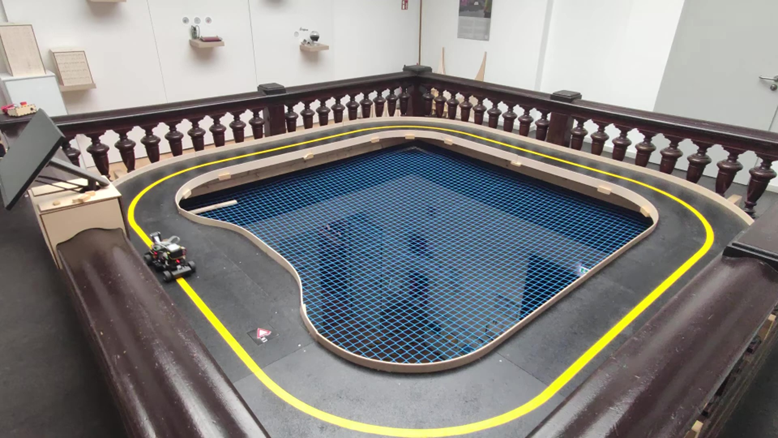
\includegraphics[scale=0.48]{track_and_car}
    \caption{Darstellung der Strecke.}
    \label{track_and_car}
\end{figure}

Die bisherige Pipeline extrahierte alle gelben
Pixel aus dem Bild und betrachtete deren dichteste Gruppierung als die
Fahrspurlinie. Der Abstand zwischen der $x$-Koordinate dieser Gruppierung und
der Mittellinie des Bildes diente als Eingabe für einen PID-Regler, der das
Fahrzeug auf die Fahrspur lenkte. 

Aufgrund der Einschränkungen der bisherigen Fahrzeugregelung, wie z. B. der
geringen maximal m"oglichen Vorwärtsgeschwindigkeit und der mangelnden
Robustheit, bestand im Vorfeld der Arbeit der Wunsch, eine neue Regelstrategie
zu implementieren. Um dieses Ziel zu erreichen, umfasst die hiererarbeitete
Lösung die Entwicklung einer neuen Bildverarbeitungspipeline und die Ersetzung des
PID-Reglers durch einen Stanley-Regler.

\chapter{Regelalgorithmus}

\section{Stanley-Regler}

In \cite{stanley} wurde im Jahr 2005 ein Regelungsalgorithmus vorgeschlagen,
der Stanley-Regler. Von den Autoren wird dieser Regler (unter Bezugnahme auf
das Auto des Rennteams Stanford University \glqq Stanley\grqq) als
\glqq Stanley-Regler\grqq bezeichnet.

Der Stanley-Regler ist ein nichtlinearer Regelungsalgorithmus, um ein
zweiachsiges Fahrzeug nur anhand der Ausrichtung des Fahrzeugs relativ zur Bahn
und der Querabweichung zu der zu verfolgenden Bahn zu steuern. Der Algorithmus hat
sich für das kinematische Modell eines zweiachsigen Fahrzeugs als asymptotisch
global stabil erwiesen. \cite{stanley}

Der Stanley-Regler ist ein Pfadfolgeregler anstelle eines
Trajektorienfolgereglers. Im Wesentlichen ist ein Pfad eine rein geometrische
Darstellung, die keinen Zeitbezug hat, während eine Trajektorie die
Zeitverläufe der Zustandskomponenten in einem bestimmten Zeitintervall
beschreibt. Als Querregler soll der Stanley-Regler das Fahrzeug auf der Bahn halten, hat aber
keinen Einfluss auf die Vorw"artsgeschwindigkeit. Dieser Ansatz ermöglicht eine
flexible Wahl der Fahrzeuggeschwindigkeit, die unter Berücksichtigung
dynamischer Effekte nach Bedarf für eine bestimmte Anwendung gewählt werden
kann. \cite{stanley}

Der Stanley-Regler wird mathematisch durch die folgende Gleichung beschrieben:
\begin{equation} 
  u = \theta - \theta_d + \arctan\left(\frac{ke_{V}}{v}\right).
  \label{eq:Stanley-Regler} 
\end{equation}
Dabei ist $u$ der Reglerausgang, welcher im Wesentlichen die "Anderung des Lenkwinkels $\varphi$
bestimmt, siehe \eqref{eq:model}, $\theta$ die aktuelle Ausrichtung des Fahrzeugs,
$\theta_d$ die Pfadausrichtung, $k$ ein Skalierungsfaktor, $v$ die
Geschwindigkeit des Fahrzeugs und $e_{V}$ die Querabweichung vom Mittelpunkt
der Vorderachse des Fahrzeugs zum Pfad. Die geometrischen Beziehungen zwischen
den Gr"o{\ss}en sind in Abb. \ref{stanley} zu sehen.

\begin{figure}[h]
    \centering
    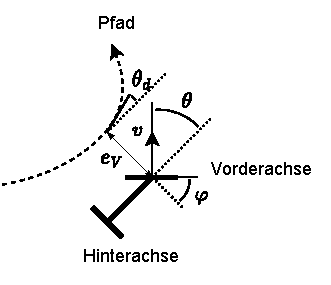
\includegraphics[scale=1.5]{stanley}
    \caption{Grafische Darstellung der geometischen Beziehungen zwischen
    den Gr"o{\ss}en des Stanley-Reglers. Der Parameter $\varphi$ bezeichnet
    den Lenkwinkel des Modellfahrzeugs.}
    \label{stanley}
\end{figure}

Der Stanley-Regler besteht aus zwei Komponenten: einer Komponente, die die
Differenz zwischen der Ausrichtung des Fahrzeugs und der des Pfades behandelt,
und einer Komponente, die die Querabweichung des Fahrzeugs vom Pfad behandelt.
Die erste Komponente, dargestellt durch $\theta_d - \theta$, beeinflusst den
Lenkwinkel so, dass er parallel zum zu verfolgenden Pfad bleibt. Die zweite
Komponente wird durch $\arctan(\frac{ke_{V}}{v})$ dargestellt und beeinflusst
den Lenkwinkel so, dass er sich auf den Pfad zubewegt, wenn sich das Fahrzeug
weiter von ihm entfernt. Zusammen bewirken diese beiden Komponenten, dass das
Fahrzeug auf den gewünschten Pfad gelenkt wird. \cite{steering-methods}


\subsection{Kleinsignalverhalten}


Um das Verhalten des Stanley-Reglers \eqref{eq:Stanley-Regler} zu verstehen,
wird der Regler um den Arbeitspunkt $\left(x_V, \theta_d\right) = \left(0,
0\right)$ linearisiert: 
\begin{equation} \bar{u} \approx \theta + \frac{k}{v}e_{V}, 
    \label{eq:linearer Stanley-Regler}
\end{equation}
wobei die Geschwindigkeit $v$ als konstant
angenommen wird. Die sich daraus ergebende Gleichung \eqref{eq:linearer
Stanley-Regler} hat die Form eines PD-Reglers. Die P-Komponente wird durch
\(\frac{k}{v}e_{V}\) gebildet. Da die Vorwärtsgeschwindigkeit des Fahrzeugs als
konstant angenommen wird, besteht eine Proportionalität zwischen den
Ableitungen von der Querabweichung \(e_{V}\) nach Zeit und Ort. Die Ableitung
von \(e_{V}\) nach dem Ort ist \(\theta\). Daher enspricht im linearisierten
Stanley-Regler die Orientierungsdifferenz \(\bar\theta\) der D-Komponente.

\subsection{Gro{\ss}signalverhalten}

Bei großen Signalen wird der Stanley-Regler durch das Verhalten der
$\arctan$-Funktion dominiert. Die Funktion $\arctan$ ist auf einen Wert zwischen
-90 und 90 Grad begrenzt und ist glatt. Das führt dazu, dass der P-Anteil des Reglers
diesen Wert nicht überschreiten kann, was der physischen Realität entspricht.

\section{Simulation}

Um ein besseres Verständnis für das Verhalten des Stanley-Reglers in einem
Modellfahrzeug zu gewinnen und auch um die Auslegung des Reglers f"ur die experimentellen
Untersuchungen vorzubereiten, wurden im Rahmen dieser Arbeit simulative Untersuchungen
des Regelkreises durchgeführt. Die Simulation umfasst drei Hauptkomponenten: den
Pfad, dem das Fahrzeug folgen muss, den Stanley-Regler und das Fahrzeugmodell.
Zur Ermittlung der Zeitreihendaten des zweiachsigen Fahrzeugs in der
Simulation wurde ein Differentialgleichungslöser eingesetzt.

Der Pfad, dem das Fahrzeug folgen muss, ist eine virtuelle Darstellung der
realen Strecke, die das Fahrzeug durchfahren wird. Eine visuelle
Darstellung der Fahrbahn findet sich in Abb. \ref{fahrbahn}. In der Simulation wird der
Pfad durch die folgende kontinuierliche statische Funktion definiert:
\begin{equation}
        \underline{p}_P(s) = (x_p, y_p, \theta_d),
\end{equation}
wobei $s$ der Eingangsparameter Kurvenl"ange ist
und $\underline{p}_P$ bzw. $(x_p, y_p, \theta_d)$ die kartesischen Koordinaten des Pfadpunkts und die
entsprechende Ausrichtung an diesem Punkt darstellen. Diese Funktion wird für
eine beliebige Anzahl von $s$-Werten diskretisiert, um eine Liste von $(x_p, y_p,
\theta_d)$-Werten zu erzeugen. Der Differentialgleichungslöser bezieht den
Stanley-Controller und das Fahrzeugmodell ein, um die Zeitreihen des
zweiachsigen Fahrzeugs unter Verwendung dieser Liste als Eingabe zu
analysieren.

\begin{figure}[h]
    \centering
    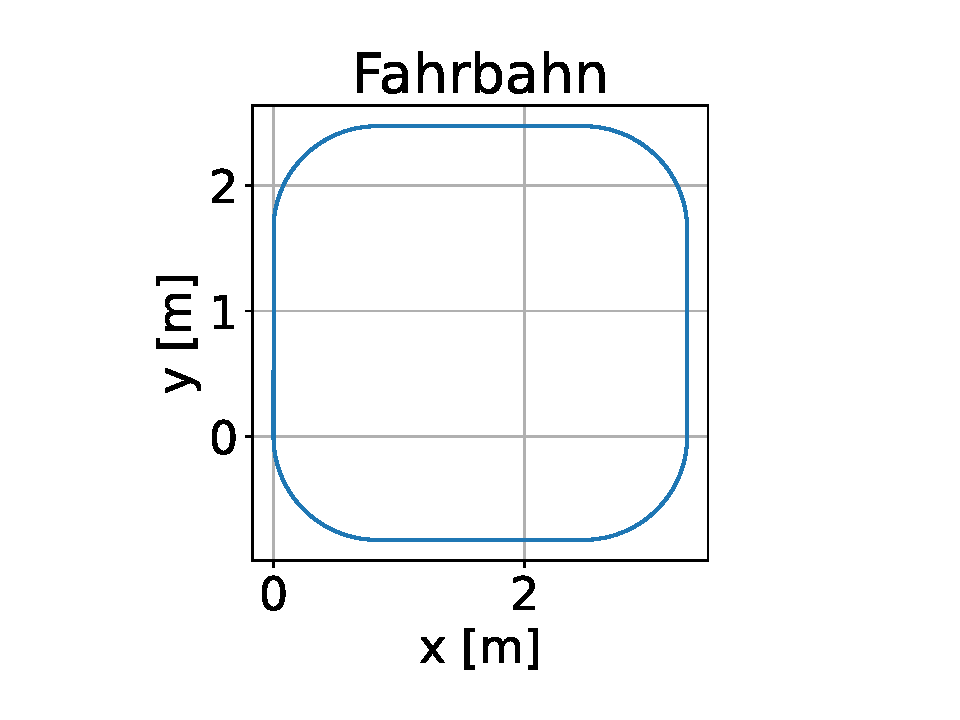
\includegraphics[scale=0.5]{fahrbahn}
    \caption{Grafische Darstellung der Fahrbahn.}
    \label{fahrbahn}
\end{figure}


Das verwendete Fahrzeugmodell ist das Modell eines zweiachsigen Fahrzeugs mit
gelenkter Vorderachse \cite{car-model}. Dieses Modell wird mithilfe der folgenden
nichtlinearen Zustandsraumdarstellung formuliert: 
\begin{subequations} \label{eq:model}
    \begin{align}
        \dot{x} &= v \cos(\theta) \\ 
        \dot{y} &= v \sin(\theta) \\ 
        \dot{\theta} &= \frac{v}{l}\tan(\varphi). 
    \end{align}
\end{subequations} 
Die Zustandskomponenten des Modells sind $x$, $y$, $\varphi$ und $\theta$, wobei
$x$ und $y$ die kartesischen Koordinaten des Mittelpunkts der Hinterachse
sind und $\theta$ die Ausrichtung des Fahrzeugs ist. $\varphi$ ist der
Lenkwinkel des Fahrzeugs. Die Eingangsgrößen des Modells sind $v$ und
$\varphi$, wobei $v$ die Geschwindigkeit des Fahrzeugs und $\varphi$ der
Lenkwinkel ist. Der Parameter $l$ bezeichnet den Abstand
zwischen der Hinterradachse und der Vorderradachse.

Der Lenkwinkel $\varphi$ ist selbst ein dynamisches System. Experimentell zeigt sich,
dass der Lenkwinkel $\varphi$ sich wie ein PT1-Glied verh"alt.
Das PT1-Glied wird durch die folgende Gleichung modelliert \cite{pt1glied}:
\begin{equation}
        \dot{\varphi} = \frac{\left(u-\varphi\right)}{T},
\end{equation}
wobei die Zeitkonstante $T$ konfiguierbar ist. Das Verhalten des Stanley-Reglers bei dynamischen Einflüssen auf den Lenkwinkel
ist von großer Bedeutung, da die globale asymptotische Stabilität des Reglers
nur für das kinematische Zweiachsmodell nachgewiesen wurde. \cite{stanley}

Da der Stanley-Regler für die Querabweichung den Mittelpunkt der Vorderachse
benötigt, muss dieser aus der Hinterachse berechnet werden. Der Mittelpunkt der
Vorderachse wird aus den Zustandskomponenten durch die folgende statische
Funktion \cite{car-model} berechnet: 
\begin{subequations}
\begin{align}
    \underline{p}_H &:= 
  \begin{bmatrix}
    x & y
  \end{bmatrix}^T \\
  \begin{bmatrix}
    x_V & y_V
  \end{bmatrix}^T
    &= \underline{p}_H + l 
  \begin{bmatrix}
    \cos(\theta + \pi/2) \\ 
    \sin(\theta + \pi/2)
  \end{bmatrix},
  \label{eq:Transformation from Rear Axle to Front Axle}
\end{align}
\end{subequations}
wobei $x_V$ und $y_V$ die kartesischen Koordinaten dieses Vorderradachsemittelpunkts sind.
Der Parameter $\underline{p}_H$ bezeichnet den Positionsvektor des Hinterradachsemittelpunkts.

Wie bereits erwähnt, besteht der Stanley-Regler aus mehreren Teilen, die
getrennt voneinander berechnet werden k"onnen. Die Ausrichtung $\theta$ ist eine
Zustandsvariable, daher ist sie unmittelbar verfügbar. Um die Querabweichung und die
Pfadausrichtung zu berechnen, muss der richtige Bahnpunkt gewählt werden. Der
Stanley-Regler verwendet den nächstliegenden Bahnpunkt vom
Vorderachsmittelpunkt des Fahrzeugs, um die Ausrichtung des Pfades $\theta_d$
und die aktuelle Querabweichung $e_{V}$ zu bestimmen. Für die Simulation wird
dieser bestimmt, indem der Punkt mit dem geringsten Abstand $\underline{\lambda}$ zum
Vorderachsmittelpunkt gefunden wird (entspricht Kurvenparameter $s^*$. An diesem Punkt wird
dann die Ausrichtung des Pfades ermittelt. Das Skalarprodukt zwischen dem
Vektor senkrecht zur Fahrzeugausrichtung $\underline{\nu}_{\perp}$ und dem Vektor
vom Pfadpunkt zur Fahrzeugvorderachse $\underline{\lambda}$ ist die
Querabweichung $e_{V}$. Zur Verdeutlichung ist in Abb. \ref{algorithm} eine visuelle
Darstellung dieser beiden Vektoren und ihres Skalarprodukts gezeigt. Die Berechnung
der wichtigen Parameter ist in folgenden Gleichungen dargestellt: \\

\begin{figure}[h]
    \centering
    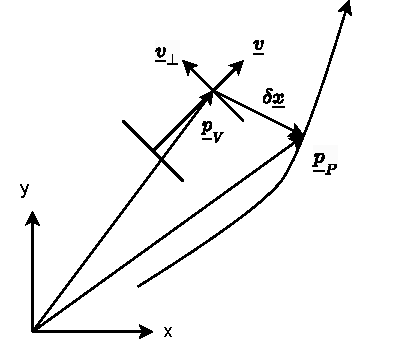
\includegraphics{dot_product}
    \caption{Grafische Darstellung der Beziehungen zwischen den ben"otigten
    Parametern. Der Vektor $\underline{p}_P(s^*)$ ist hier der Pfadpositionsvektor mit dem
    kleinsten Abstand zum Vorderradachsemittelpunkt.}
    \label{algorithm}
\end{figure}

\begin{subequations}
\begin{align}
    \underline{\nu} &:= \begin{bmatrix} \cos(\theta) & \sin(\theta) \end{bmatrix}^T, \\
        \underline{\nu}_{\perp} &:= \begin{bmatrix} \cos(\theta + \pi/2) & \sin(\theta + \pi/2) \end{bmatrix}^T, \\
            s^* &:= \arg\min_{s}  \left\Vert\underline{p}_V - \underline{p}_P(s) \right\Vert_2, \\
    \underline{\lambda} &:= \underline{p}_P(s^*), \\
    e_{V} &:= \underline{\lambda} \cdot \underline{v}_{\perp}.
 \label{alg:quer}
\end{align}
\end{subequations}

Die Pfadausrichtung und die Querabweichung werden dann an den Stanley-Regler "ubergeben,
und der Ausgang des Reglers wird in das Fahrzeugmodell eingespeist. Ein
Übersichtsdiagramm des Regelkreises ist in Abb. \ref{control_loop} dargestellt.

\begin{figure}[h]
    \centering
    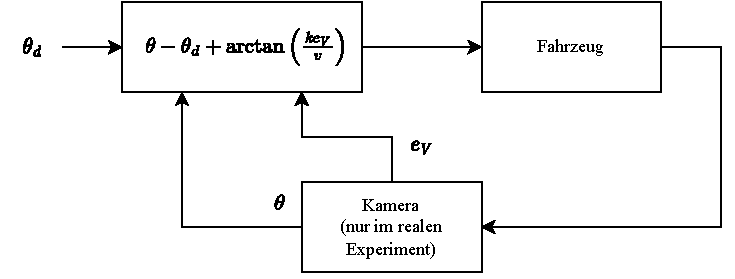
\includegraphics[scale=1.2]{control_loop}
    \caption{Darstellung des Regelkreises.}
    \label{control_loop}
\end{figure}

Der nominelle Stanley-Regler \eqref{eq:Stanley-Regler}
arbeitet mit zeitkontinuierlichen Signalen, die sich von den
vom \glqq echten\grqq Fahrzeug verwendeten zeitdiskreten Signalen
unterscheiden. Das Fahrzeug nimmt Bilder mit einer festen Abtastfrequenz auf,
die von der Pipeline verarbeitet werden, bevor sie in den Regler eingespeist
werden (n"aheres dazu in den Kapiteln 3 und 4). Um dieses Verhalten zu simulieren, wird ein Speicher in den Simulator
eingebaut, um die Ausrichtung und die Querabweichung zu speichern. Der
Stanley-Regler verwendet dann diese zwischengespeicherten Werte für eine
bestimmte Dauer. Dieser Speicher-Ansatz ahmt das Verhalten eines Halteglieds
nullter Ordnung nach, und die Ausgabe dieses Haltegliedes wird anschließend in
den Stanley-Regler eingespeist. Dieser Simulationsansatz ermöglicht die
Untersuchung des Fahrzeugverhaltens für verschiedene Abtastfrequenzen. Von
besonderer Bedeutung ist die Stablit"at des Regelkreises mit verschiedenen
Abtastfrequenzen. Der Vergleich der Simulationsergebnisse bei
verschiedenen Abtastfrequenzen ist in Abb. \ref{sampling} dargestellt. 

\begin{figure}[h]
    \centering
    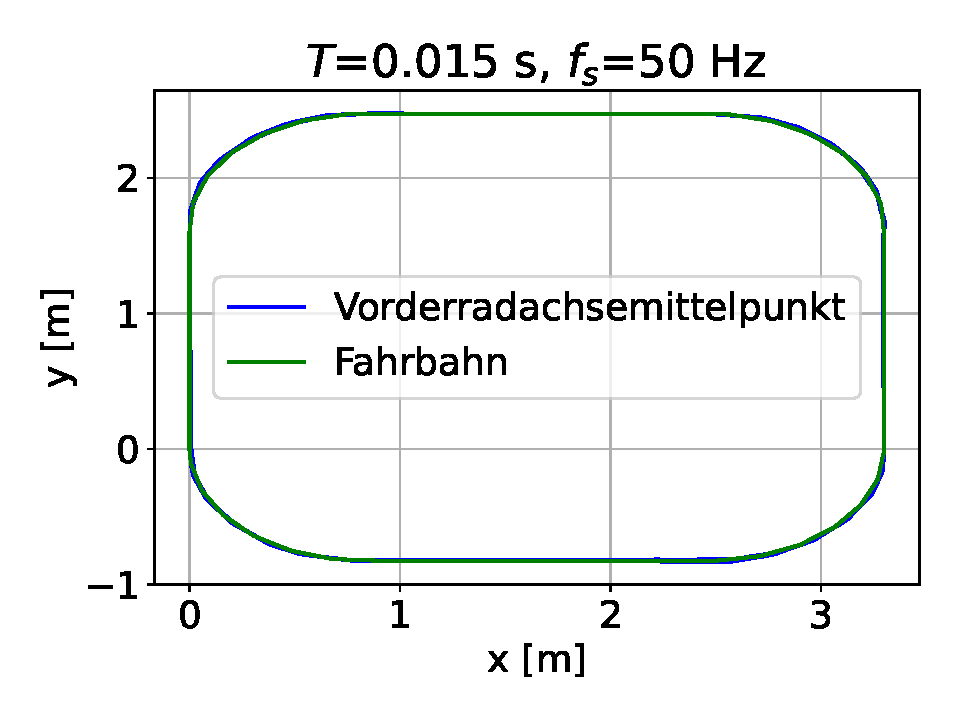
\includegraphics[scale=0.47]{0.015ms50Hz}
    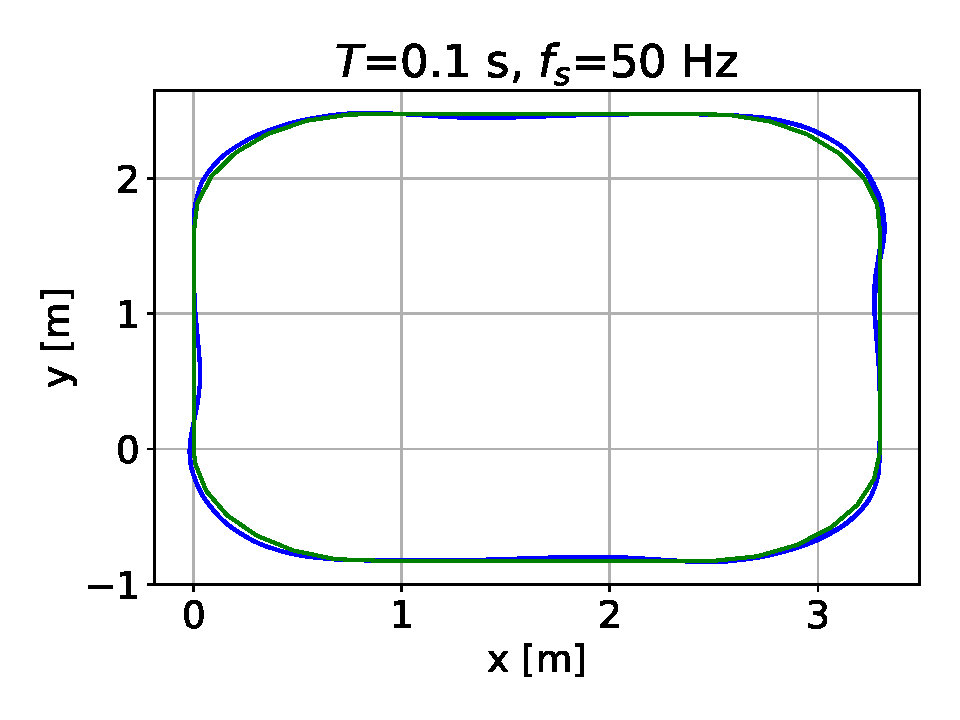
\includegraphics[scale=0.47]{0.1ms50Hz}
    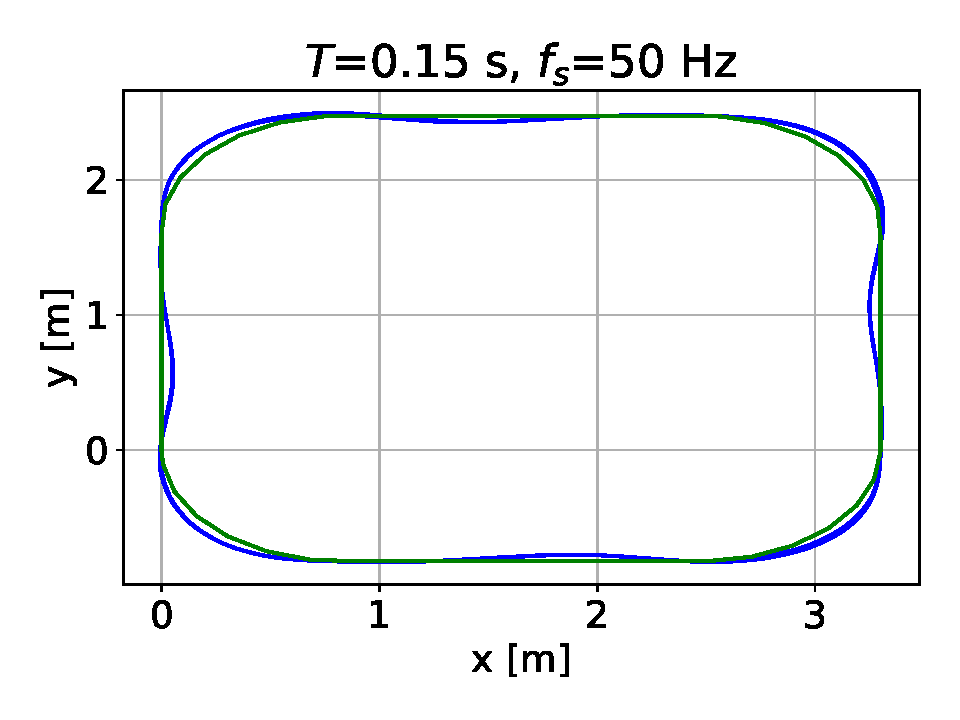
\includegraphics[scale=0.47]{0.15ms50Hz}
    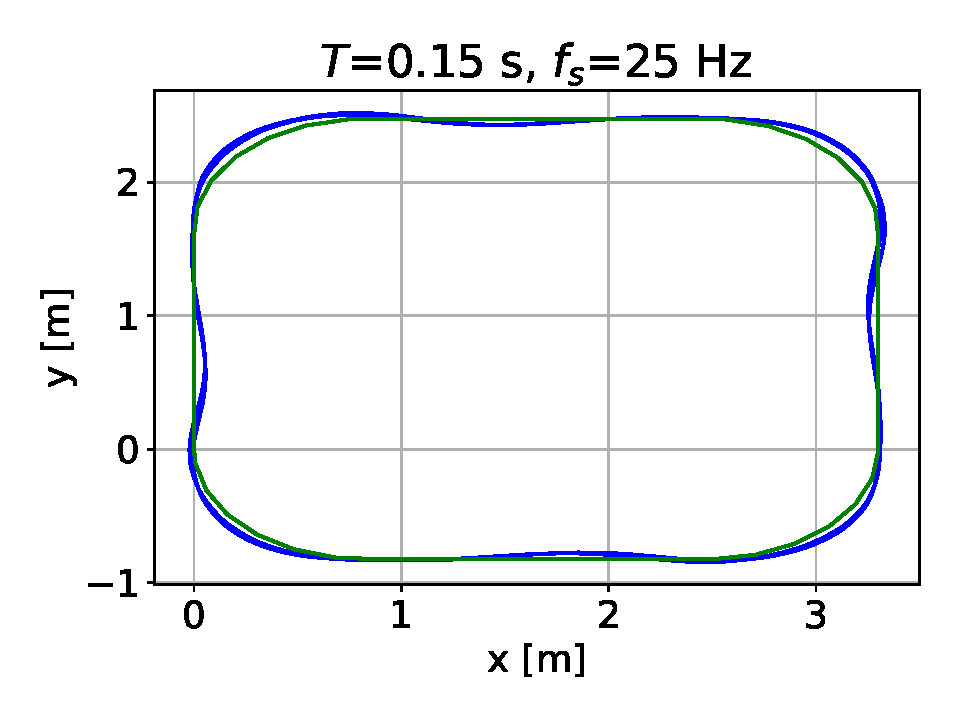
\includegraphics[scale=0.47]{0.15ms25Hz}
    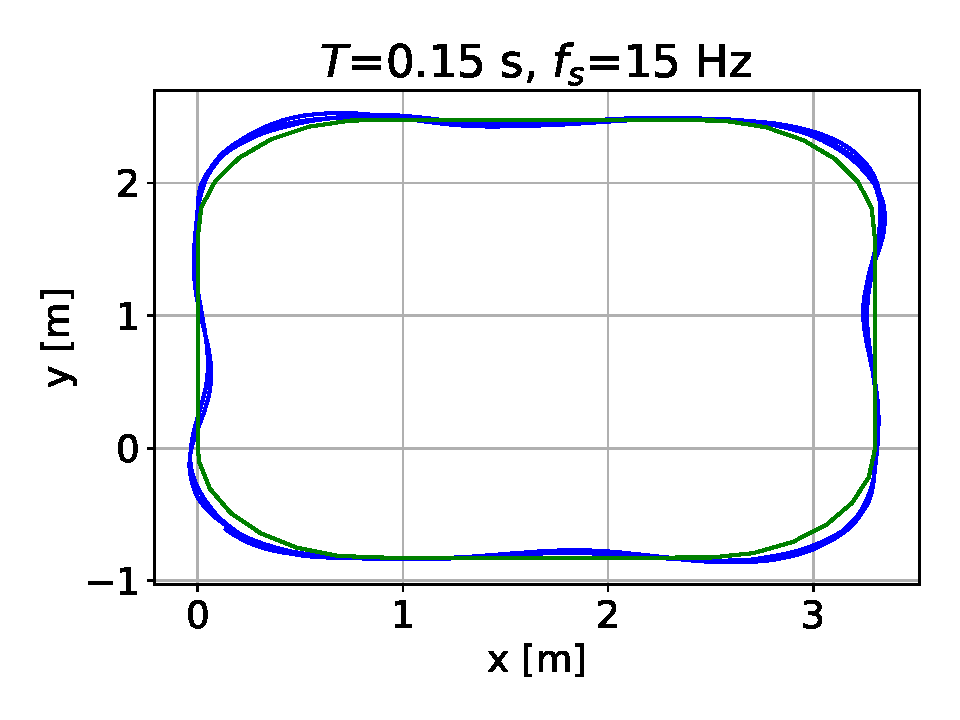
\includegraphics[scale=0.47]{0.15ms15Hz}
    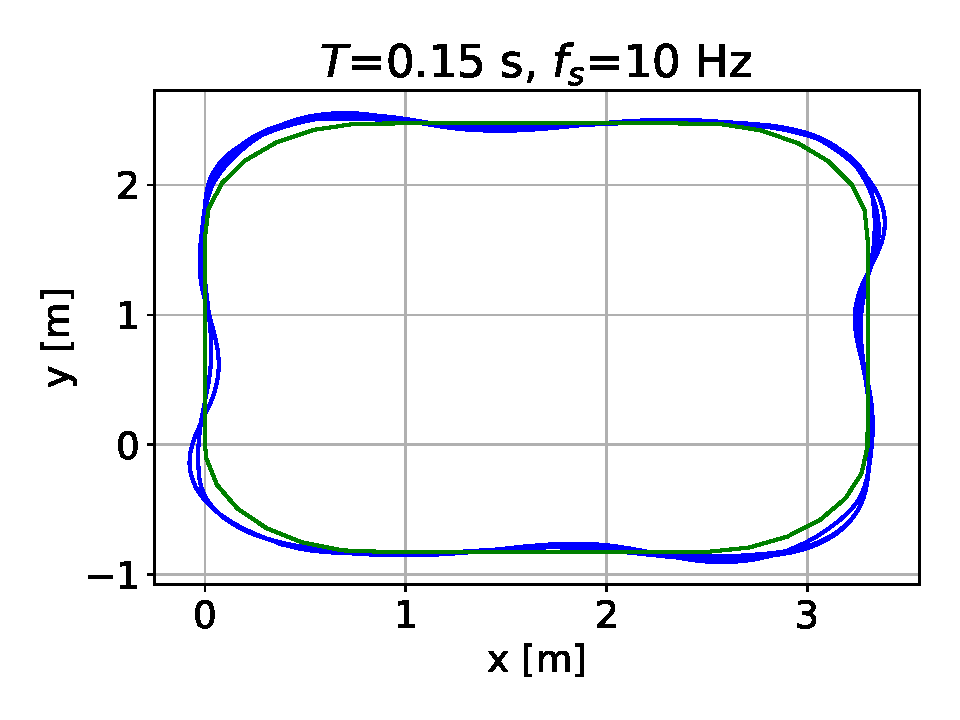
\includegraphics[scale=0.47]{0.15ms10Hz}
    \caption{Verhalten des Stanley-Reglers bei verschiedenen Abtastfrequenzen und Zeitkonstanten.
    Das Verhalten bleibt "ahnlich bei Frequenzen unter 15 Hz. Der Stanley-Regler folgt den Pfad besser
    wenn die Zeitkonstante des PT1-Glieds niedrig ist, aber die Lenkwinkelstrecke im Auto hat eine 
    Zeitkonstante zwischen 100 und 200 ms.}
    \label{sampling}
\end{figure}

Wie in Abb. \ref{sampling} ersichtlich, wird der Stanley-Regler durch die Abtastfrequenz
beeinflusst, wobei bei niedrigeren Frequenzen ein deutlicher Effekt zu
beobachten ist. Oberhalb eines Schwellenwerts von 15 Hz scheint das
Verhalten des Fahrzeugs jedoch nicht wesentlich durch die Abtastfrequenz
beeinflusst zu werden. 


\chapter{Bildverarbeitung}

Im Vergleich zu dem vorher verwendeten PID-Regler benötigt der
Stanley-Regler zusätzliche Informationen, nämlich die Ausrichtung des Pfades.
Die neue Bildverarbeitungspipeline ist darauf ausgelegt, diese notwendigen
Informationen zu extrahieren. Der beschriebene Prozess basiert auf \cite{addison-pipeline}. Wie in Abb. \ref{pipeline} zu sehen, besteht die
Pipeline aus mehreren Schritten zur Berechnung der Ausrichtung und der
Querabweichung. Im Folgenden werden die einzelnen Schritte der Bildverarbeitung
genauer beschrieben. \\

\begin{figure}[h]
    \centering
    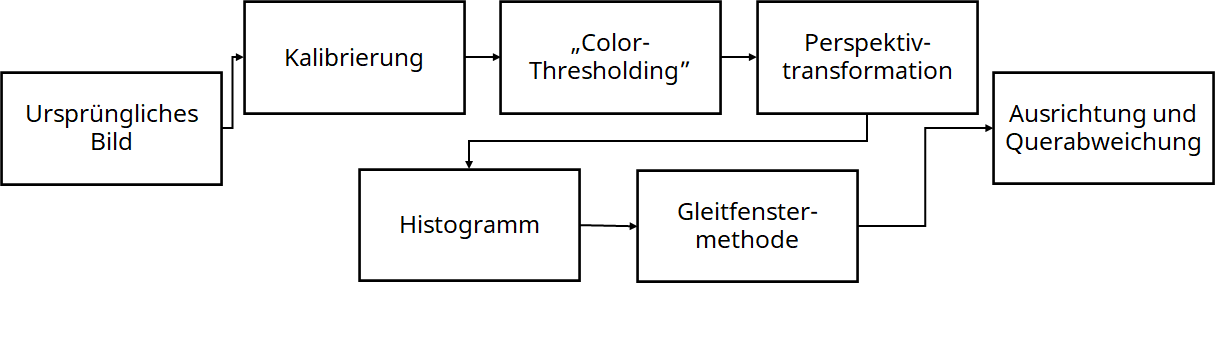
\includegraphics[scale=0.72]{pipeline}
    \caption{Grafische Darstellung des Bildverarbeitungspipelines.}
    \label{pipeline}
\end{figure}


\section{Verzeichnungskorrektur}
Für die CoRoLa
Car Platform wurde eine Fischaugenkamera gewählt. Der Vorteil einer
Fischaugenkamera ergibt sich aus ihrem größeren Blickwinkel im Vergleich zu
einer normalen Kamera. Eine Fischaugenkamera hat eine sog. \glqq
tonnenförmige Verzeichnung\grqq \cite{wiki-verzei}, wodurch gerade Linien
gekrümmt werden. Die Krümmung dieser Linien hängt von ihrem radialen Abstand
vom Bildmittelpunkt ab. Ein Beispiel ist in Abb. \ref{barrel} zu sehen. Diese
Verzeichnung kann mit Hilfe der Software \cite{opencv} auf Grundlage einer 
Kamerakalibrierung kompensiert werden.

\begin{figure}[h]
    \centering
    \fbox{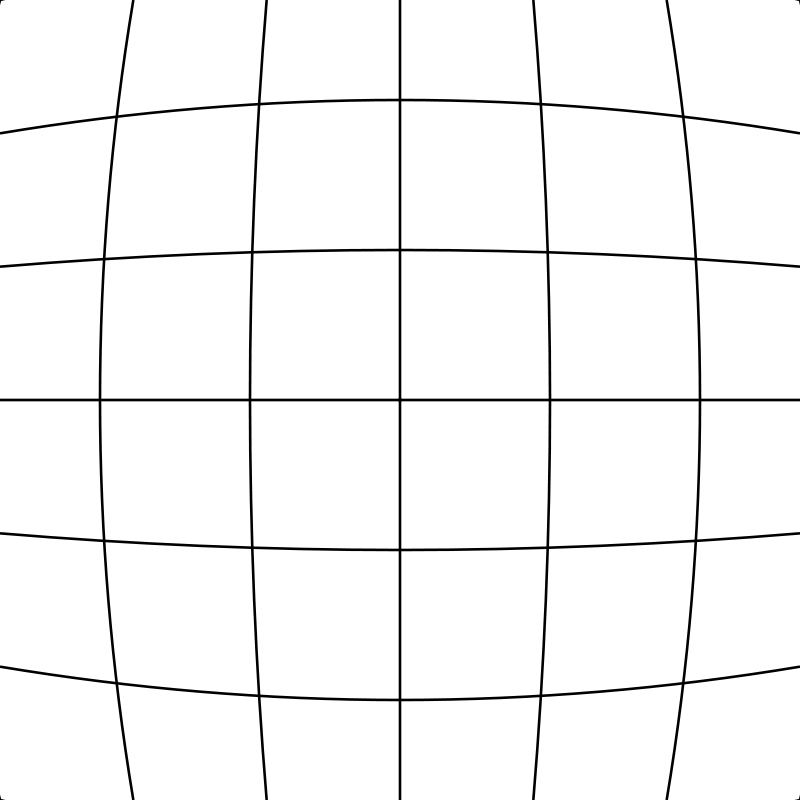
\includegraphics[scale=0.175]{Barrel_distortion}}
    \caption{Ein Beispiel einer tonnenf"ormigen Verzeichnung.}
    \label{barrel}
\end{figure}

Diese ist notwendig, um die extrinsischen und intrinsischen
Parameter der Kamera n"ahrungsweise zu bestimmen. 

\subsection{Kalibrierung}

Die intrinsischen Parameter
einer Kamera werden häufig durch die 3x3-Matrix 
\begin{equation} 
    K = 
    \begin{bmatrix} 
        f_x & 0 & c_x\\ 
        0 & f_y & c_y\\ 
        0 & 0 & 1
    \end{bmatrix}, 
\end{equation} 
\glqq Kameramatrix\grqq dargestellt, wobei $f_x$ und $f_y$ die Brennweiten der Kamera in Pixeln in den
Richtungen $x$ und $y$ sind und $c_x$ und $c_y$ die Koordinaten des Bildmittelpunkts
bezeichnen. Die extrinsischen Parameter werden häufig durch die folgende Matrix
dargestellt: 
\begin{equation}
    \begin{bmatrix} R & T \end{bmatrix}. 
\end{equation} 
Dabei ist $R$ die Rotationsmatrix der Kamera in Bezug auf das dem Experiment zugrunde 
liegenden Bezugskoordinatensystem und $T$
der Positionsspaltenvektor des Ursprungs des Bezugssystem, ausgedrückt in den
Koordinaten des Kamerabildes. Die \glqq Kameratransformationsmatrix\grqq $M$ ist die Abbildung von
den Weltkoordinaten auf Pixelkoordinaten, die durch die
Matrix-Matrix-Multiplikation dargestellt wird, 
\begin{equation} 
    M = K 
    \begin{bmatrix} 
        R & T
    \end{bmatrix}. 
\end{equation} 
Durch das Rekonstruieren der $M$-Matrix mit Hilfe von Software \cite{opencv} kann das verzerrte
Bild wieder in das Bezugssystem des Experiments "uberf"uhrt werden, wodurch gekrümmte Linien gerade
werden.

Im Einzelnen l"auft der Prozess folgenderma{\ss}en ab: eine Kamera wird anhand
einer Sammlung von Fotos mit bekannten geraden Linien kalibriert. In der Regel
wird eine Reihe von Schachbrettbildern mit bekannten Dimensionen verwendet.
\cite{addison} Danach werden Fotos des Schachbretts in verschiedenen Winkeln
und in verschiedenen Positionen relativ zur Kamera aufgenommen. Diese
Bilderserie wird dann in den Algorithmus zur Kamerakalibrierung eingespeist,
der zunächst die Positionen der Schachbrettfelder und der sie verbindenden
Linien bestimmt.  Die Anzahl der benötigten Bilder hängt von
der jeweiligen Kamera ab, eine große Sammlung von Fotos führt jedoch zu einer
genaueren Annäherung an die wirklichen Parameter.  Die Verwendung von Bildern mit einer
höheren Auflösung führt ebenfalls zu genaueren Parametern. \cite{addison} Die
angenäherten Parameter sind jedoch nur g"ultig für die Verarbeitung von Bildern,
die mit der gleichen Auflösung aufgenommen wurden wie die für die
Kalibrierung verwendeten Bilder. Um die Kameramatrix für Bilder mit einer
niedrigeren Auflösung zu verwenden, muss die intrinsische Kameramatrix $K$ mit
der folgenden Formel skaliert werden: 
\begin{equation} 
    K_n = k K, 
\end{equation} 
wobei $k$ ein positiver skalarer Wert ist, der den Skalierungsfaktor darstellt
\cite{scalingK} . Da es sich bei der intrinsischen Kameramatrix um eine affine
Abbildung handelt, muss der Wert bei $K_{\mathrm{n},3, 3}$ auf 1 gesetzt
werden. Die resultierende intrinsische Kameramatrix funktioniert bei kleineren
Auflösungen, die dem Seitenverhältnis der für die Kalibrierung verwendeten
Bilder gleich sind. 

\subsection{Korrektur}

Nach der erfolgten Kalibrierung gleicht der Algorithmus anhand des Modells der
Fischaugenkamera die Verzeichnung aus. Wie in Abb. \ref{checkerboards} zu
sehen, sind beispielsweise die gekrümmt abgebildeten Linien des Schachbretts nach der
Kalibrierung wieder begradigt.

\begin{figure}[h]
    \centering
    \fbox{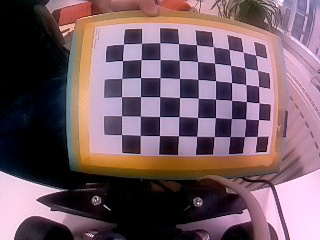
\includegraphics[scale=0.75]{before_calibration_checkerboard}}
    \fbox{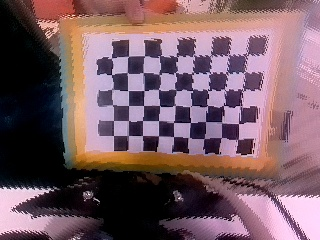
\includegraphics[scale=0.75]{after_calibration_checkerboard}}
    \caption{Die Kalibrierung des linken Bilds liefert das rechte Bild. Die gekr"ummte Linie 
    des Schachbretts sind gerade nach dem Verzeichnungskorrektur. Der Grund f"ur die
    wellenf"ormigen Verzerrungen ist die nicht perfekte Kalibrierung.} 
    \label{checkerboards}
\end{figure}

Ein Nachteil der Verzeichnungskorrektur ist, dass jedes korrigierte Bild eine
geringere Auflösung hat als das Originalbild. Dies ist eine Folge des
Korrektursprozess  da dieser einen Teil des Bildes verzerrt,
insbesondere die Pixel nahe den Ecken des Bildes. Daher werden diese Pixel beim
Korrektursprozess aus dem resultierenden Bild entfernt. Um das Bild in
seiner ursprünglichen Auflösung zu rekonstruieren, wird eine Interpolation
verwendet. Die Interpolation liefert jedoch ein unschärferes Bild als das
Original. Um dies zu kompensieren, empfiehlt es sich grunds"atzlich, eine Kamera mit
hochauflösenden Bildern zu kalibrieren und dann Bilder mit dieser Auflösung
aufzunehmen. Anstatt den Interpolator zu verwenden, verkleinert man die Bilder
dann auf eine Auflösung, die für die jeweilige Anwendung ausreichend ist.  Das
Ergebnis ist ein genaueres Bild ohne Unschärfe. Leider ist dieser Prozess sehr
rechenintensiv, und es wurde beschlossen, nur die Bilder aus dem Interpolator
zu verwenden, um die Rechenleistung der Pipeline zu erhöhen.

Ein weiterer Nachteil der Verzeichnungskorrektur ist, dass sich der Mittelpunkt der
Kamera verschieben kann. Ein Beispiel dafür ist in Abb. \ref{shifted} zu sehen. Durch
manuelles Ändern von $c_x$ kann der Bildmittelpunkt wieder an seine
ursprüngliche Position verschoben werden. 

\begin{figure}[h]
    \centering
    \fbox{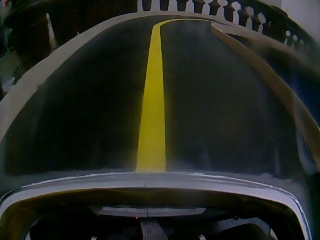
\includegraphics[scale=0.5]{orig_not_shifted}}
    \fbox{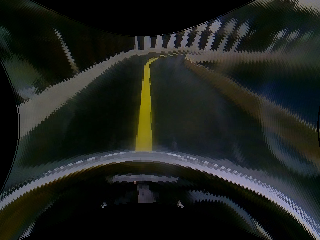
\includegraphics[scale=0.5]{cal_shifted}}
    \caption{Ein Beispiel von dem Korrekturschritt. Die Mittellinie im
    rechten Bilds ist leicht nach rechts verschoben.}
    \label{shifted}
\end{figure}

\section{\glqq Color-Thresholding\grqq}

Als Nächstes folgt der Schritt des sogenannten \glqq Color-Thresholding\grqq. In diesem
Schritt werden alle Pixel aus dem Bild entfernt, die nicht zur Bahnlinie geh"oren.
In dieser Implementierung sind alle Farbe au{\ss}er Gelb unerw"unscht.

Zunächst wird das Bild von allen Pixeln ohne hohen Rotanteil gefiltert, da
Hellgelb im Rot-Grün-Blau-Farbraum (RGB) einen hohen Rotanteil hat.
Anschließend wird das Bild in den HSV-Farbraum (Hue, Saturation, Value engl. f"ur Farbwert, Sättigung und
Helligkeitswert) umgewandelt. 

Im RGB-Farbraum ist reines Gelb so definiert, dass sowohl der rote als auch der
grüne Kanal gleich sind und der blaue Kanal auf Null gesetzt ist. Dies lässt
nur einen Freiheitsgrad für die Justierung der Pipeline zu.  Ein einziger
Freiheitsgrad führt zu Problemen bei der Abstimmung, da die Pipeline dadurch
weniger in der Lage ist, Schwankungen zu berücksichtigen. Unterschiedliche
Lichtverhältnisse oder reflektierende Oberflächen sind Beispiele für solche
Störungen.

Im HSV-Farbraum bestimmt der Farbwertkanal die Farbe, der Sättigungskanal die
Reinheit des Farbtons und der Wertekanal die Helligkeit des Farbtons.
\cite{hsv} Nach der Auswahl des Intervalls von Farbwerten, in diesem Fall
innerhalb des gelben Bereichs, werden der Helligkeits- und der Sättigungskanal
verwendet, um den spezifischen Gelbton auszuwählen. Die Verwendung dieser
beiden Kanäle ermöglicht eine zuverlässigere Erkennung der Farbe.

Um die gelbe Spur zu erkennen, filtert die Pipeline Farben außerhalb des gelben
Farbtonbereichs heraus und schneidet dann den unteren Teil des Helligkeits- und
Sättigungskanals ab. Das Ergebnis ist, dass nur reines Gelb im Bild übrig
bleibt. Die in der Pipeline verwendeten Werte für Gelb werden in Tab.
\ref{hsvtable} dargestellt. \\

\begin{table}[h]
\begin{center}
\begin{tabular}{|c|c|c|c|}
\hline
    & H & S & V\\
\hline
\hline
    Minimaler Wert & 15 & 90 & 90 \\
\hline
    Maximaler Wert & 40 & 255 & 255 \\
\hline
\end{tabular}
    \caption{Minimalen und Maximalen Werte f"ur die Bestimmung des gelben Farbtonbereiches. Der Bereich
    der Werte sind zwischenn 0 und 255 begrenzt.}
    \label{hsvtable}
\end{center}
\end{table}

Das Ergebnis dieses Schritts der Pipeline ist f"ur ein Beispielbild in Abb.
\ref{color-thresholding} dargestellt. Um die Darstellung zu vereinfachen,
werden die gelben Pixel hier und im Folgenden als schwarze Pixel auf wei{\ss}em
Grund dargestellt. Als Eingabe bekommt die Pipeline ein kalibriertes Bild und 
gibt dann nur Pixel aus, die zur Bahnlinie geh"oren. \\

\begin{figure}[h]
    \centering
    \fbox{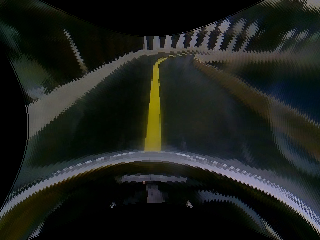
\includegraphics[scale=0.5]{calibrated}}
    \fbox{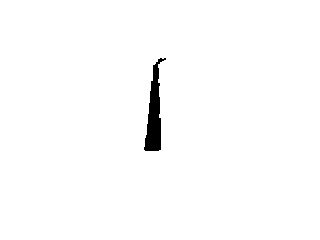
\includegraphics[scale=0.5]{thresholded}}
    \caption{Ein Beispiel von der Ausgabe des Color-Thresholdings. Links: Bild
    nach dem Kalibrierungsschritt, Eingang zum \glqq Color-Thresholding\grqq.
    Rechts: bin"ares Bild mit nur Pixeln, die als gelb erkannt wurden.}
    \label{color-thresholding}
\end{figure}

\section{Perspektivtransformation}

Der dritte Teil der Bildverarbeitungspipeline ist die Perspektivtransformation. 
Die Kamera steht nicht senkrecht zur Bahn, wie es bei einer idealen
Draufsicht der Fall wäre, sondern die Blickrichtung bildet einen Winkel von ca.
30° zur Bahnebene.

Wenn ein Bild mit einer am Fahrzeug montierten Kamera aufgenommen wird, ist die
Fahrbahn nicht rechteckig, sondern trapezförmig. Diese Perspektive
erfordert, dass alle Berechnungen bezüglich der Fahrspurlinie deren scheinbar abnehmende
Breite kompensieren müssen. Um dies zu vermeiden, wird eine
Perspektivtransformation durchgeführt. 

Bei der Perspektivtransformation wird eine Teilmenge des Bildes ausgeschnitten
und so angepasst, dass sie das gesamte Bild f"ullt. Im allgemeinen Fall muss
diese Scherung nicht das gesamte Bild umfassen, sondern sie kann in einen
anderen Bildausschnitt "ubertragen werden. Ein Beispiel ist in Abb.
\ref{roi-pt} dargestellt. Mithilfe dieser Perspektivtransformation wird die
trapezförmige Form der Fahrbahnlinie zu einer rechteckige Form korrigiert. \\

\begin{figure}[h]
    \centering
    \fbox{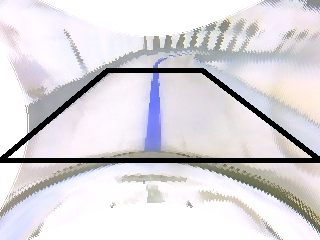
\includegraphics[scale=1.0]{roi_inverted.png}}
    \fbox{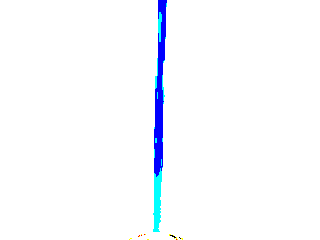
\includegraphics[scale=0.5]{perp_trans.png}}
    \caption{Perspektivtransformation f"ur ein Beispielbild. Die Trapez im linken
    Bild wird ausgeschnitten und gestreckt, sodass sich das rechte Bild ergibt.
    Zu diesem Zeitpunkt hat noch kein \glqq Color-Thresholding\grqq stattgefunden.}
    \label{roi-pt}
\end{figure}

Eine Folge dieser neuen Perspektive ist, dass das resultierende Bild einer
Draufsicht ähnelt. Die Perspektivtransformation vereinfacht auch die weitere
Bildverarbeitung, da alle Objekte außerhalb des Trapezes abgeschnitten werden
und nur die Spur übrig bleibt. Wie in Abb. \ref{roi-pt} zu sehen ist, führt die
Perspektivtransformation jedoch zu farblichen Artefakten im Bild. Daher ist es
erforderlich, dass dieser Schritt nach dem \glqq Color-Thresholding\grqq-Schritt
erfolgt.

\section{Histogramm}

Nach der Perspektivtransformation wird ein Histogramm der schwarzen Pixel
erstellt, um den Startpunkt für die im n"achsten Schritt folgende
Gleitfenstermethode zu bestimmen. Die Anzahl der schwarzen Pixel wird für jede
Spalte des Bildes gezählt, und diese Zahlen werden in einer Liste gespeichert.
Es wird davon ausgegangen, dass die Spalten mit den höchsten Zahlen
Fahrspurinformationen enthalten, und der Index der Spalte mit der höchsten Zahl
wird als Startpunkt für die Gleitfenstermethode gewählt. Dieser Schritt trägt
dazu bei, die Berechnungszeit zu verkürzen, indem Teile des Bildes
herausgefiltert werden, die keine Fahrspurinformationen enthalten. Eine
visuelle Darstellung des Histogramms ist in Abb. \ref{hist} zu sehen. \\

\begin{figure}[h]
    \centering
    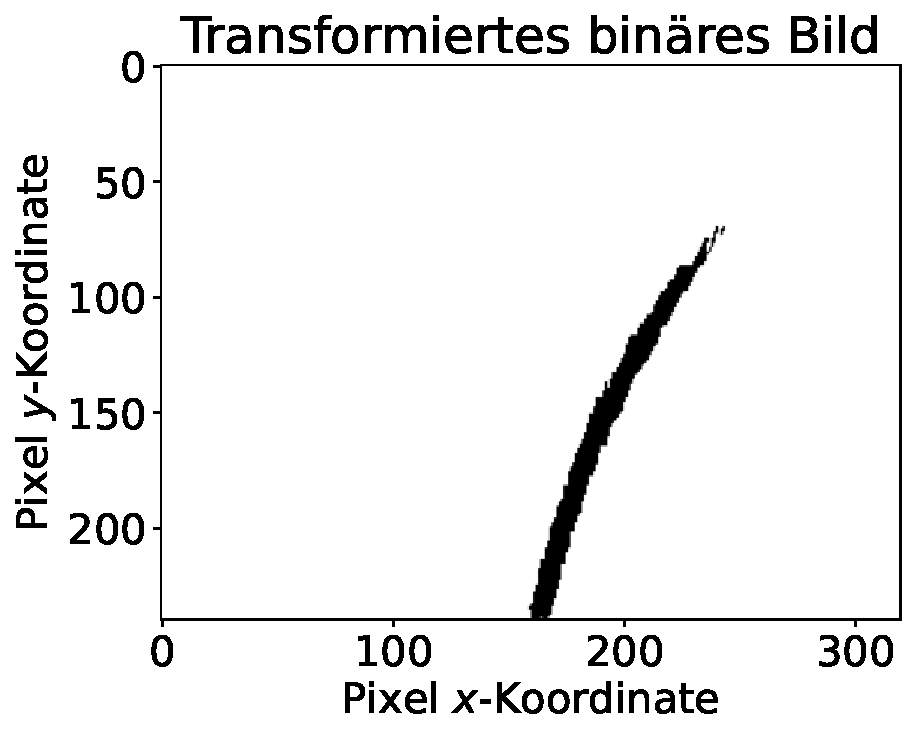
\includegraphics[scale=0.47]{hist1}
    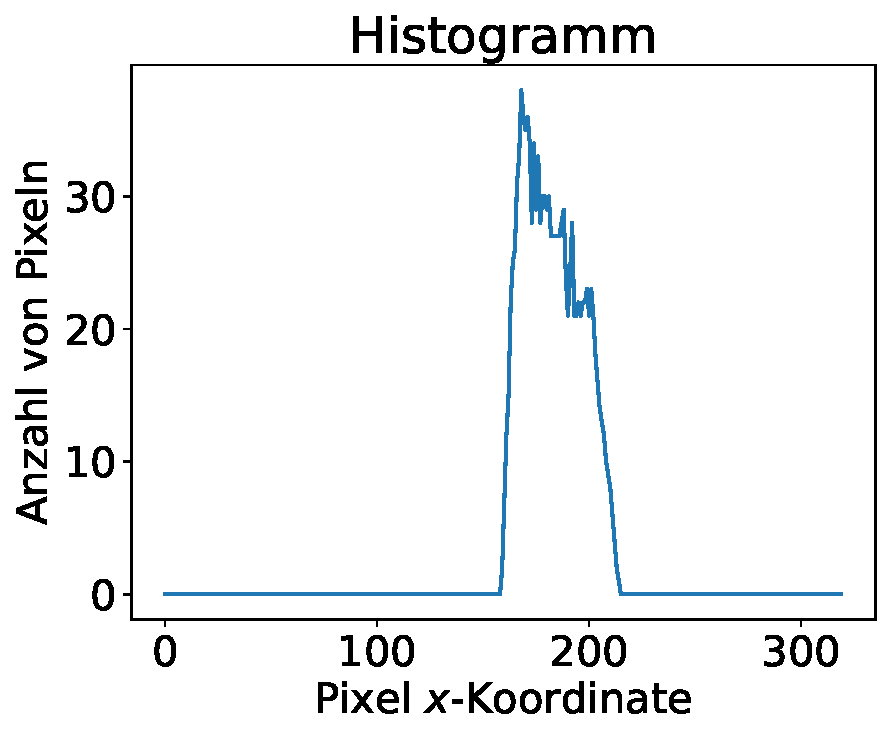
\includegraphics[scale=0.47]{hist2}
    \caption{Histogramm der schwarzen Pixel. Die Spitze des Histogramms liegt bei dem
    $x$-Schnittpunkts.}
    \label{hist}
\end{figure}

\section{Gleitfenstermethode}

Im fünften Schritt der Pipeline wird die Form der Fahrspur bestimmt. Dazu soll
in einem vorbereitenden Schritt das Bild bereinigt werden, indem Pixel gelöscht
werden, die klar nicht zu der gesuchten Fahrspur gehören. Dies wird durch die
Verwendung der Gleitfenstermethode erreicht, die in \cite{addison-pipeline}
beschrieben ist.

Dabei wird eine ausgewählte Anzahl von Rechtecken (Fenstern) erstellt. Die Höhe
wird so gewählt, dass die Summe der H"ohe aller Rechteck gleich der Bildh"ohe
ist, während ihre Breite entsprechend proportional zur Bildbreite gewählt wird.
Die Anzahl der Fenster wird so gewählt, dass der aus dem Histogramm bekannte
Bereich der schwarzen Pixel umfasst wird, wie in Abb. \ref{gleit} zu sehen ist. 

Als zweiter Schritt wird die $x$-Koordinate des Mittelpunkts des ersten Fensters auf den
Spitzenwert des Histogramms aus dem vorherigen Schritt gesetzt. Dann wird die
Anzahl der schwarzen Pixel innerhalb des Fensters gezählt. Wenn die Anzahl über
einem gewählten Schwellenwert liegt, werden die Pixel zu einem Array
hinzugefügt und der Mittelwert der $x$-Koordinaten dieser Pixel berechnet. Die
$x$-Koordinate des nächsten Fensters wird auf diesen berechneten Mittelwert
gesetzt und um die Breite der Fenster in $y$-Richtung verschoben. Dieser
Vorgang wird dann für alle verbleibenden Fenster wiederholt. Wenn in einem
Fenster nicht gen"ugend schwarze Pixel enthalten sind, wird das Fenster
ignoriert und das folgende Fenster darüber gelegt.  

Die Pixel, die nicht innerhalb der einzelnen Fenster liegen, werden dann aus
dem Bild herausgefiltert. Das Bild vor und nach dem Filterungsprozess ist in
Abb. \ref{gleit} zu sehen. Mit Hilfe der Methode der kleinsten Quadrate wird ein
Polynom 2. Ordnung durch die verbleibenden Pixel approximiert.

Um das Polynom, das die Fahrspur repräsentiert, aus den $n$ verbleibenden
Pixeln zu bestimmen, wird die folgende Berechnung \cite{lstsq} verwendet:
\begin{subequations}
\begin{align}
    \underline{x} &:= \begin{bmatrix} x_1 & x_2 & ... & x_n \end{bmatrix}^T \\
        \bold{Y} &:= \begin{bmatrix} 1 & y_1 & y_1^2 \\ 1 & y_2 & y_2^2 \\ \vdots & \vdots & \vdots \\ 1 & y_n & y_n^2 \end{bmatrix} \\
            \underline{\hat{\beta}} &:= \begin{bmatrix} \hat{\beta_0} & \hat{\beta_1} & \hat{\beta_2} \end{bmatrix}^T \\
                \underline{\hat{\beta}} &= \left(\bold{Y}^T\bold{Y}\right)^{-1}\bold{Y}^T\underline{x},
\end{align}
\end{subequations}
wobei $\underline{x}$ und $\underline{y}$ die Vektoren sind, die die $x$- und
$y$-Koordinaten der übrigen Pixel enthalten. $\hat{\beta_0}$, $\hat{\beta_1}$ und
$\hat{\beta_2}$ sind die Koeffizienten des approximierten Polynoms. 

Unter Verwendung der approximierten Koeffizienten erhält man die folgende Gleichung:
\begin{equation}
    \hat{x} = \hat{\beta_0} + \hat{\beta_1}y + \hat{\beta_2}y^2,
    \label{poly}
\end{equation}
wobei $y$ die $y$-Koordinate und $\hat{x}$ die angenäherte $x$-Koordinate der
Fahrspur ist. Die Gleichung liefert eine analytische Darstellung der Fahrspur. 

\begin{figure}[h]
    \centering
    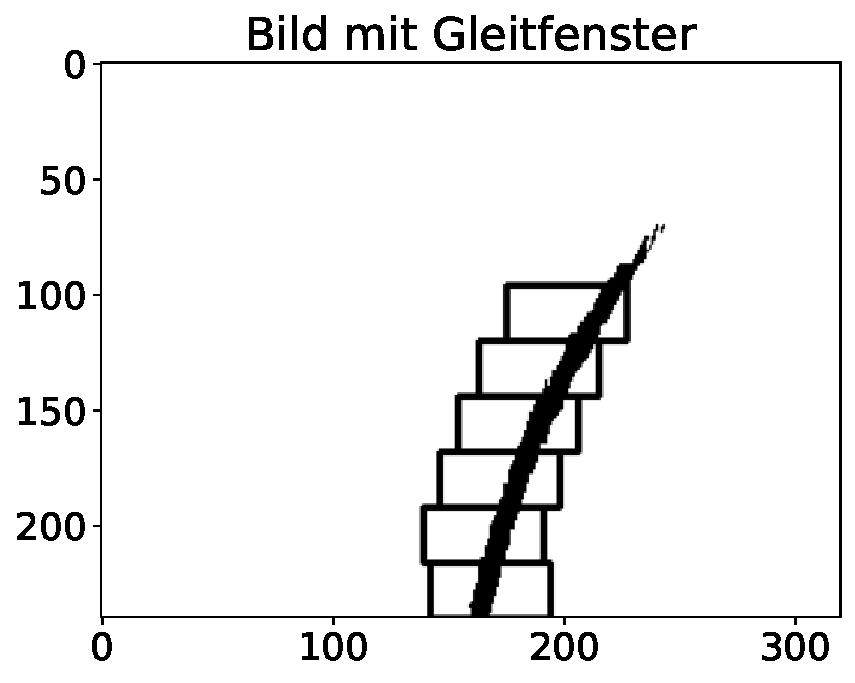
\includegraphics[scale=0.47]{before_filter}
    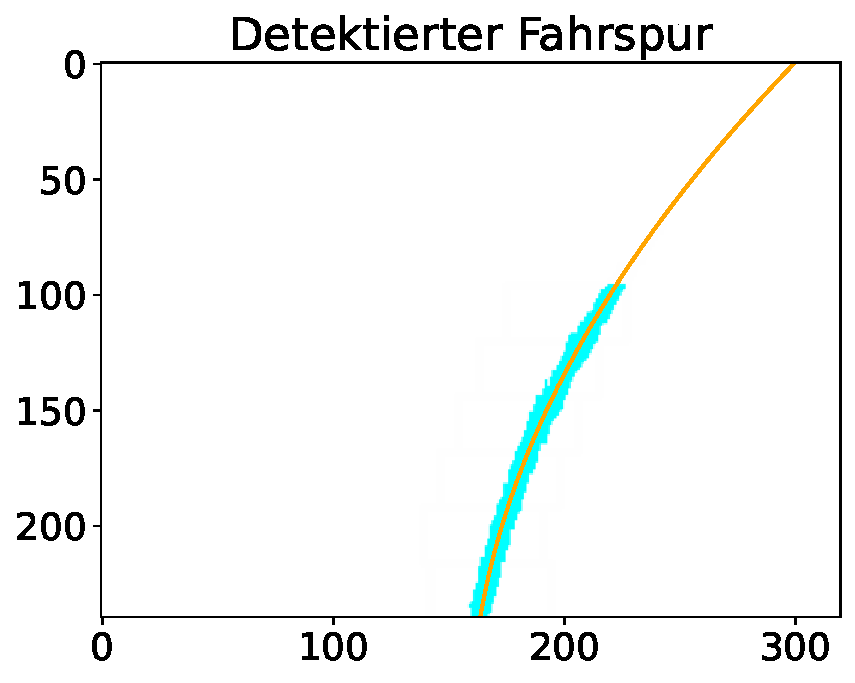
\includegraphics[scale=0.47]{after_filter}
    \caption{Das linke Bild ist ein Beispiel von der Gleitfenstermethode. Das rechte Bild
    zeigt das Polynom, das von den verbleibenden Pixel approximiert wurde.}
    \label{gleit}
\end{figure}

\section{Berechnung von Ausrichtung und Querabweichung}

In dem letzten Schritt der Pipeline werden die Ausrichtung des Fahrzeugs und die Querabweichung von
der Fahrspurlinie berechnet. 

Aus dem in dem vorangegangenen Schritt berechneten Polynom \eqref{poly} wird eine
analytische Ausrichtung an einem ausgewählten Punkt entlang der Bahn mit der
folgenden Gleichung \cite{tangentangle} ermittelt:
\begin{subequations} 
    \begin{align}
        \hat{x} &= g(y), \\
        \theta &= \arctan(g^\prime(y)).
    \end{align}
\end{subequations} 
Der Arkustangens der Ableitung des Polynoms liefert die Ausrichtung der Spur
an einem bestimmten Punkt. Für den Stanley-Regler wird nur die Differenz
zwischen der Bahnausrichtung und der Ausrichtung des Fahrzeugs benötigt. Da
kein globales Koordinatensystem für das Fahrzeug benötigt wird, kann die
Ausrichtung des Fahrzeugs zu jedem Zeitpunkt als $0^{\circ}$ definiert
werden. Die aus dem Bild erkannte Ausrichtung $\theta$ der Bahn bildet somit
direkt die für den Stanley-Regler relevante Winkel-Eingangsgröße.

Die Abweichung von der Fahrspurlinie wird aus dem angepassten Polynom mit
folgender Funktion berechnet: 
\begin{equation}
    e_{V} = \left(\frac{w}{2} - f(h)\right)\cdot \sigma_\mathrm{mpp}.
\end{equation}
Dabei ist $w$ die Breite des Bildes, $e_{V}$ der Abstand des Fahrzeugs zur
Fahrspur, $\sigma_\mathrm{mpp}$ eine Skalierungskonstante zur Umrechnung von
Pixeln in Meter und $g(h)$ die Ausgabe des berechneten Polynoms am unteren Rand
des Bildes, d.h. bei $y=h$. Zusammenfassend wird die Differenz aus der
$x$-Komponente des Mittelpunkts und der $x$-Komponente des Polynompunkts am
unteren Bildrand von Pixel in Meter umgerechnet.

\section{Ausrei{\ss}er}

Fahrspurerkennungalgorithmen k"onnen zu einem Phänomen führen, das als \glqq
Ausreißer\grqq bekannt ist. Diese treten auf, wenn der Algorithmus die
Fahrspurlinie in einem bestimmten Bild falsch bestimmt. Abb. \ref{ausrei} zeigt
eine Sequenz von drei Einzelbildern, wobei das erste Einzelbild (links) den
Ausgangspunkt bildet. Im ersten Bild wird die Fahrspurlinie richtig erkannt,
aber im zweiten Bild tritt ein Ausreißer auf, bei dem die Fahrspurlinie falsch
bestimmt wird. Im letzten Bild wird die Fahrspurlinie wieder korrekt erkannt.

\begin{figure}[h]
    \centering
    \fbox{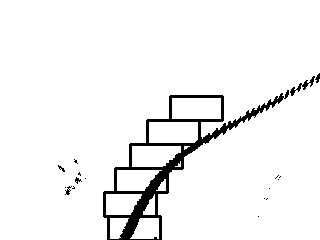
\includegraphics[scale=0.8]{before_outlier}}
    \fbox{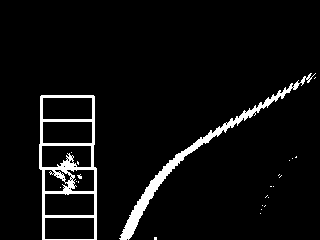
\includegraphics[scale=0.8]{outlier}}
    \fbox{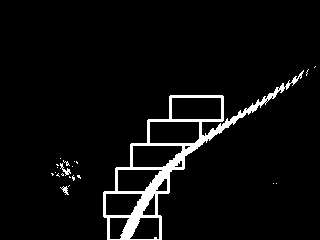
\includegraphics[scale=0.8]{after_outlier}}
    \caption{Ein Beispiel von einem Ausrei{\ss}er. Die drei Bilder wurden
    nacheinander aufgenommen. Im rechten und linken Bilder wurde die Fahrspur
    richtig erkannt. Im mittleren Bild wurde die Fahrspur falsch erkannt.}
    \label{ausrei}
\end{figure}

Eine der Hauptursachen für Ausreißer ist die falsche Auswahl der HSV-Werte im Color-Thresholding-Schritt.
Wenn die im Algorithmus verwendeten HSV-Werte nicht restriktiv genug sind,
werden Farben außer Gelb möglicherweise nicht herausgefiltert, was zu einer
ungenauen Bestimmung der Fahrspurlinie führt.

Außreißer sind ein unvermeidbares Resultat des Bildverarbeitungsprozesses. Die Empfindlichkeit mit der ein
Regelungsalgorithmus auf sie reagiert ist ein wichtiges Kriterium bei der Wahl eines Algorithmus.
Wie in Kapitel 4 genauer beschrieben, erschien in den hier durchgeführten Tests der Stanley-Regler
in dieser Hinsicht weniger empfindlich als der PID-Regler.


\iffalse
\section{Pipeline-Optimierungen}

Bei der Entwicklung der Bildverarbeitungspipeline wurde festgestellt, dass die
Laufzeit der Pipeline zu gro{\ss} war. Um die Rechenzeit der Pipeline auf ein
akzeptables Niveau zu verbessern, wurde eine Optimierung eingeführt. Weitere
Optimierungen sind zwar möglich, würden aber den Rahmen der Arbeit sprengen und
werden daher hier nicht behandelt.

Das Python-Programm cProfiler wurde verwendet, um die Funktionsaufrufe der
Pipeline mit ihren jeweiligen Laufzeiten zu untersuchen. Da es sich bei der
Pipeline um ein deterministisches Programm handelt, verbessert die
Zwischenspeicherung der Ausgabe der teuren Funktionsaufrufe im Speicher die
Laufzeit der Pipeline. Daher wird bei allen nachfolgenden Pipeline-Ausführungen
das zwischengespeicherte Ergebnis zurückgegeben, anstatt die Berechnung erneut
auszuführen. Beispielsweise ist die Berechnung der perspektivischen
Transformationsmatrizen kostspielig, was bei der Zwischenspeicherung zu einer
Leistungssteigerung der Pipeline führt. Diese Zwischenspeicherung hat die Laufzeit 
des Pipelines vom X ms zu Y ms verringert.

Um die Leistungsverbesserung der Pipeline zu beweisen, wurde ein Experiment
durchgeführt. Zunächst wird die Pipeline einmal ausgeführt und die Laufzeit
ignoriert, da die Leistungsverbesserung nur für nachfolgende Ausführungen der
Pipeline relevant ist. Daher wird bei der zweiten Ausführung der Pipeline die
Laufzeit für beide Pipeline-Varianten gemessen, mit und ohne
Zwischenspeicherung der teuren Funktionsaufrufe aus der ersten Ausführung. Das
Experiment wird dann 100 Mal durchgeführt und das Ergebnis tabellarisch
erfasst. Das arithmetische Mittel der Laufzeiten für beide Varianten wird dann
miteinander verglichen, um die Laufzeitverbesserung zu messen. Das Experiment
zeigte, dass das Zwischenspeichern dieser Funktionsaufrufe die Laufzeit von X
ms auf Y ms senkte. (Ich muss die Werte nochmal finden.)
\fi

\chapter{Experimentelle Untersuchungen}
\section{Hardware}

Die CoRoLa-Car-Platform besteht aus einem busförmigen Modellfahrzeug mit einem Raspberry Pi, 
einer Fisheye-Kamera,
einem b"urstenlosen Gleichstrommotor und einem Motorregler zur Steuerung der
Fahrzeuggeschwindigkeit und einem Servomotor um den Radeinschlag des Fahrzeugs
zu steuern. Der Raspberry Pi sendet Power-Werte-Signale an den
Motorregler und den Servoregler, um das Fahrzeug zu steuern. 

\begin{figure}[h]
    \centering
    \fbox{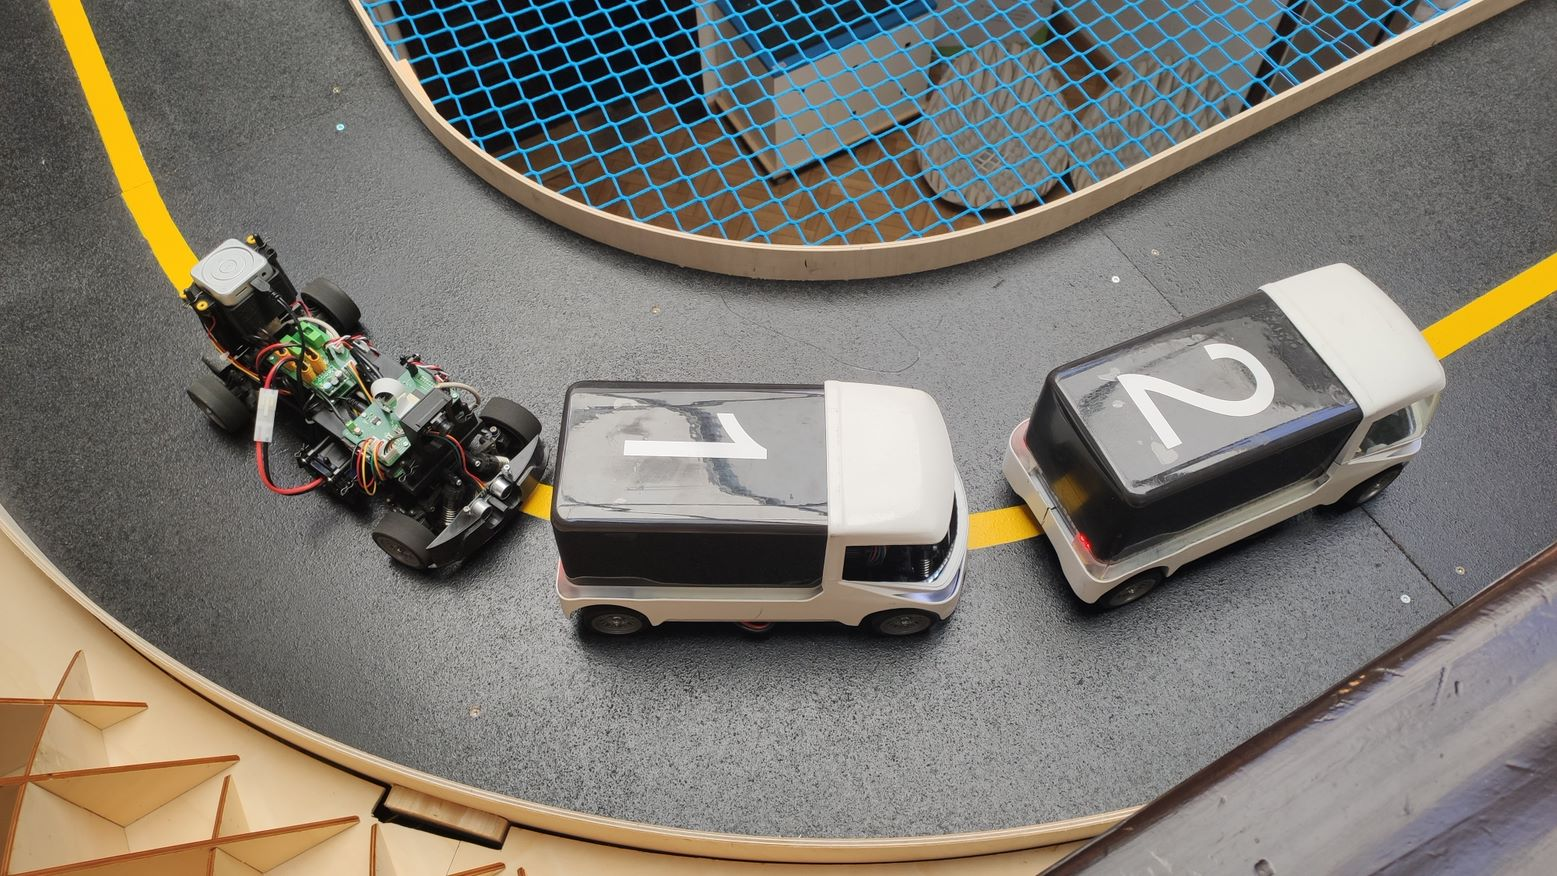
\includegraphics[scale=0.2]{cars}}
    \caption{Modellfahrzeuge.}
    \label{cars}
\end{figure}


\section{Experimentkriterien}

\subsection{H"ochstgeschwindigkeit}

Um die Höchstgeschwindigkeit zu messen, fährt das Fahrzeug mit einer bestimmten
Vorwärtsgeschwindigkeit auf der Strecke. Wenn das Verhalten des Fahrzeugs als
\glqq akzeptabel\grqq angesehen wird, wird das Fahrzeug angehalten und die
Geschwindigkeit erhöht. Dieser Vorgang wird so lange wiederholt, bis das
Verhalten des Fahrzeugs nicht mehr \glqq akzeptabel\grqq ist. Das \glqq
akzeptable\grqq Verhalten des Fahrzeugs wird empirisch anhand der folgenden
beiden Kriterien definiert: Fähigkeit, der Fahrspur grunds"atzlich zu folgen, 
d.h. nicht mit der Randbegrenzung zu kollidieren, und Ausbleiben von
beobachteten Schwingungen.

\subsection{Maximal m"oglicher Fehlerwinkel}

Die maximalen Fehlerwinkel sind definiert als die maximalen Winkel, bei denen
das Fahrzeug in der Lage ist, den Weg links bzw. rechts der Fahrspurlinie
wiederzufinden. Um dies zu messen, wird das Fahrzeug bei deaktiviertem
Motorregler parallel zur Fahrspurlinie platziert. Dann wird das Fahrzeug
im Uhrzeigersinn gedreht, wobei der Ausgang des jeweiligen Reglers in Echtzeit
angezeigt wird. Das Fahrzeug wird so lange gedreht, bis der Ausgang des Reglers
entweder den plausiblen Gültigkeitsbereich verlässt oder konstant Null ist.
In beiden Fällen ist das Fahrzeug nicht mehr in der Lage die Spur zu wiederzufinden.

\subsection{Bahnfolgeverhalten}

Die Messung des Fahrzeugversatzes erfolgt durch die folgenden zwei Versuche.
Zunächst fährt das Fahrzeug mit einer bestimmten Vorwärtsgeschwindigkeit auf
der Strecke. Dabei wird mit einer Überwachungskamera ein Video von der
Kurvenfahrt des Fahrzeugs aus der Vogelperspektive aufgenommen. Das Fahrzeug
wird bei unterschiedlichen Vorwärtsgeschwindigkeiten aufgezeichnet. Bei der
ersten Aufnahmerunde wird das Fahrzeug mit dem Stanley-Regler gesteuert, bei
der zweiten mit dem PID-Regler. Dieses Experiment wird für die gewählten
Geschwindigkeiten von 1,0, 1,25, 1,5, 1,75 und 2,0 Metern pro Sekunde
durchgeführt.

\subsection{Reglerausgang}

Um den Reglerausgang der beiden Regler zu messen, wird das Fahrzeug dreimal die 
vollständige Strecke abfahren gelassen. Während der Fahrt wird der
Ausgang des Reglers aufgenommen. Nach der Fahrt werden die Daten im Zeitverlauf
grafisch dargestellt und der zeitliche Mittelwert der Daten angegeben.
Dies ist sinnvoll, 
da für das Fahren von Kurven immer ein bestimmtes Stellsignal für den Lenkwinkel anliegen muss. 
Zu erwarten wäre ein periodischer Signalverlauf, da es sich um eine geschlossene Bahn handelt.

\section{Ergebnisse}

\subsection{H"ochstgeschwindigkeit}

Wenn der PID-Regler für das Modellfahrzeug verwendet wird, führen
Geschwindigkeiten von mehr als 1,5 $\frac{\mathrm{m}}{\mathrm{s}}$ zu einer
geringeren Robustheit. Im Gegensatz zum Stanley-Regler bringt der PID-Regler
das Fahrzeug zum Schwingen, wenn ein Ausreißer auftritt, und benötigt mehr
Zeit, um auf die Spur zurückzukehren. Das Schwingungsverhalten nimmt mit der
Vorwärtsgeschwindigkeit des Fahrzeugs zu. Wenn die Geschwindigkeit 2,0
$\frac{\mathrm{m}}{\mathrm{s}}$ übersteigt, steuert der PID-Regler das Fahrzeug
gegen die Wand des Streckenaufbaus. Selbst Geschwindigkeiten zwischen 1,5 und 1,75
$\frac{\mathrm{m}}{\mathrm{s}}$ erfordern eine Überwachung durch einen Menschen,
um Kollisionen zu vermeiden. Dieser muss das Fahrzeug vor der Spurwand manuell mit 
einem Notaus stoppen.

Im Vergleich dazu benötigt der Stanley-Regler keine Überwachung, bis die
Vorwärtsgeschwindigkeit des Fahrzeugs 2,3 $\frac{\mathrm{m}}{\mathrm{s}}$ erreicht. Bei höheren
Geschwindigkeiten weicht das Fahrzeug jedoch immer weiter von der gewünschten
Bahn ab. Dabei oszilliert es um die gelbe Fahrspur ohne je wieder für einen längeren
Zeitraum genau auf die Spur zu gelangen.

\subsection{Maximal m"oglicher Fehlerwinkel}

Die Ergebnisse des Experiments sind in Tab. \ref{fehlerwinkel} zu sehen.
Der Stanley-Regler ist im Vergleich zum PID-Regler weniger tolerant gegenüber
einer Abweichung von der Fahrspur. Dies liegt an dem Kalibrierungsschritt der
Pipeline und der Anforderung eines approximierten Polynoms, was es für den
Stanley-Regler schwieriger macht, die Fahrspur zu erkennen. Im Gegensatz dazu
benötigt der PID-Regler nur eine Gruppe von gelben Pixeln im Bild.

\begin{table}[h]
\begin{center}
\begin{tabular}{|c|c|c|}
\hline
    & PID (\textdegree) & Stanley (\textdegree)\\
\hline
\hline
    Uhrzeigersinn & 75 \pm 1& 50 \pm 1 \\
\hline
    Gegenuhrzeigersinn & 54 \pm 1 & 44 \pm 1 \\
\hline
\end{tabular}
    \caption{Maximal m"oglicher Fehlerwinkel beider Regler, wenn das Fahrzeug im oder gegen den Uhrzeigersinn
    gedreht wird.}
    \label{fehlerwinkel}
\end{center}
\end{table}

Der Stanley-Controller benötigt für die Gruppierung der gelben Pixel eine
bekannte Geometrie, typischerweise in Form einer Linie oder eines
Kurvenabschnitts, während der PID-Controller keine solchen Voraussetzungen hat.

\subsection{Bahnfolgeverhalten}

Abb. \ref{ab:1.0} und \ref{ab:1.25} zeigen, dass die beiden Regler sich bei niedrigeren
Vorw"artsgeschwindigkeiten "ahnlich verhalten. Aber Abb.
\ref{ab:1.5}, \ref{ab:1.75} und \ref{ab:2.0} zeigen, dass der PID-Regler bei
h"oheren Vorw"artsgeschwindigkeiten die Bahn genauer verfolgt als der
Stanley-Regler. Selbst unter Berücksichtigung des anfänglichen Versatzes bringt
der Stanley-Regler das Fahrzeug erst am Ende der Kurve auf die Fahrspur,
während der PID-Regler das Fahrzeug mit einer leichten nach links driftenden
Bewegung, die mit der Vorwärtsgeschwindigkeit skaliert, auf der Bahn hält.

Die Ergebnisse der Simulation des Stanley-Reglers in Abb. \ref{sampling} mit
einer Vorwärtsgeschwindigkeit von 1,75 $\frac{\mathrm{m}}{\mathrm{s}}$ und einer Abtastfrequenz von 50 Hz
stimmen mit dem Verhalten des Stanley-Reglers auf der tatsächlichen Strecke weitgehend 
überein. Allerdings driftet der Stanley-Regler, wie in der Abb. \ref{ab:2.0} gezeigt,
vor der Kurve vom geraden Streckenabschnitt weg. Dieses Ph"anomen wird als \glqq Drift
\grqq bezeichnet.

Im Rahmen der Arbeit wurde versucht, diesen Drift zu kompensieren, aber trotz der
Anpassung des Bezugspunkts für die Querabweichung blieb der Drift bestehen.
Eine manuelle Änderung des Referenzpunktes führte dazu, dass das Fahrzeug bei
der Fahrt im oder gegen den Uhrzeigersinn um die Strecke unterschiedliche
Parameter benötigte, was nicht praktikabel war. Daher wurde der Drift vorerst
so belassen, wie er ist. In Kapitel 5 werden mögliche Anpassungen des
Stanley-Reglers erörtert, die seine Leistung in Zukunft verbessern könnten.

\begin{figure}[h]
    \begin{subfigure}{0.5\textwidth}
        \centering
        \fbox{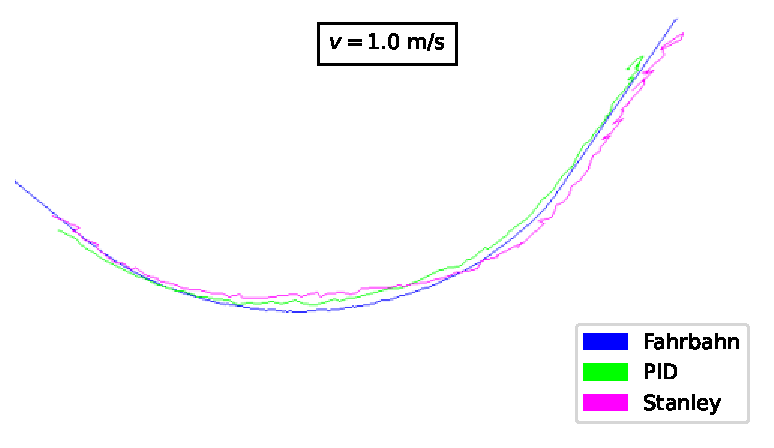
\includegraphics[width=0.85\linewidth]{done1.0}}
        \caption{$v = 1.0 \frac{\mathrm{m}}{\mathrm{s}}$.}
        \label{ab:1.0}
    \end{subfigure}
    \begin{subfigure}{0.5\textwidth}
        \centering
        \fbox{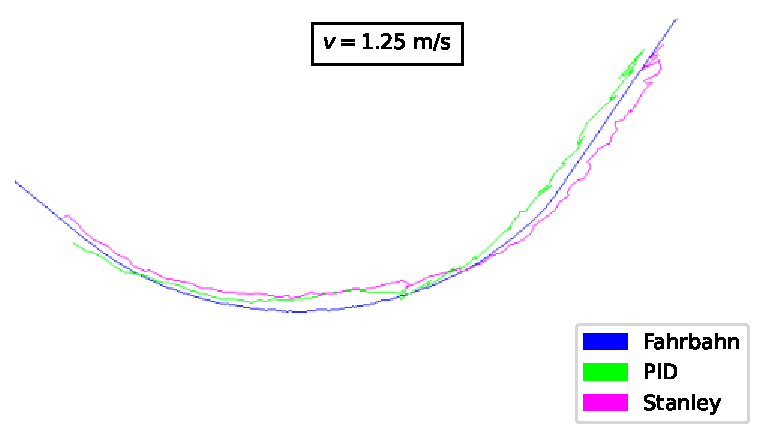
\includegraphics[width=0.85\linewidth]{done1.25}}
        \caption{$v = 1.25 \frac{\mathrm{m}}{\mathrm{s}}$.}
        \label{ab:1.25}
    \end{subfigure}
    \caption{Gezeigt ist der vom Fahrzeug gewählte Pfad (Fahrtrichtung von
    rechts nach links) f"ur die Vorw"artsgeschwindigkeiten $v = 1.0
    \frac{\mathrm{m}}{\mathrm{s}}$ und $v = 1.25
    \frac{\mathrm{m}}{\mathrm{s}}$. Dabei wurde der Standort des Fahrzeugs
    nicht immer ganz korrekt erfasst, was zu den sichtbaren Zacken
    führt. Es ist sichtbar, dass der PID- und der Stanley-Regler ungef"ahr
    das gleiche Verhalten haben.}
\end{figure}
\begin{figure}[h]
    \centering
    \begin{subfigure}{0.4\textwidth}
        \centering
        \fbox{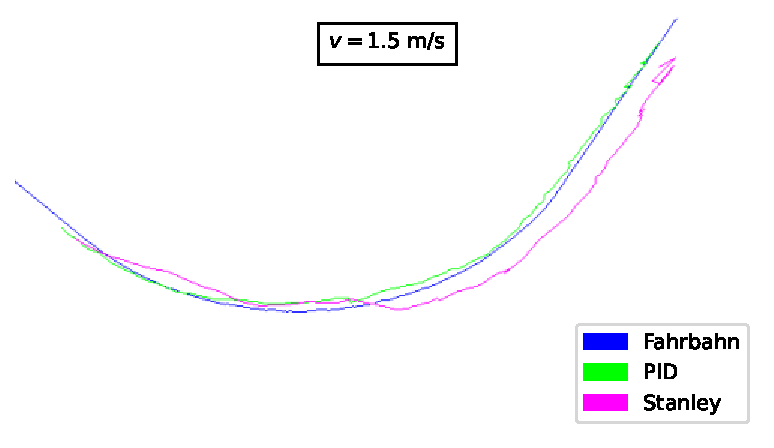
\includegraphics[width=0.9\linewidth]{done1.5}}
        \caption{$v = 1.5 \frac{\mathrm{m}}{\mathrm{s}}$.}
        \label{ab:1.5}
    \end{subfigure}
    \begin{subfigure}{0.4\textwidth}
        \centering
        \fbox{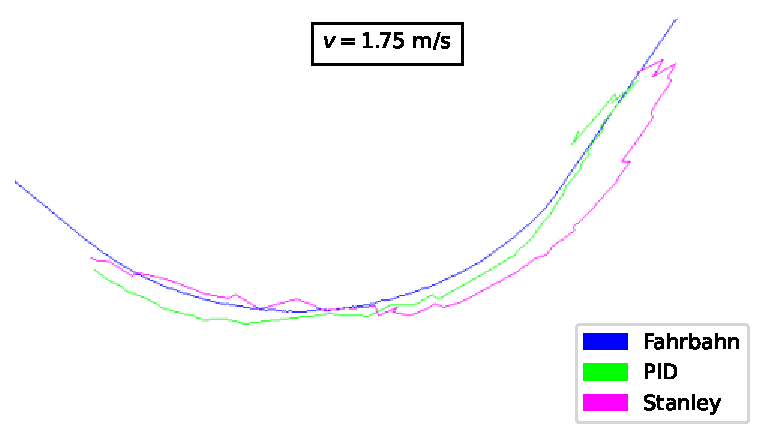
\includegraphics[width=0.9\linewidth]{done1.75}}
        \caption{$v = 1.75 \frac{\mathrm{m}}{\mathrm{s}}$.}
        \label{ab:1.75}
    \end{subfigure}
    \begin{subfigure}{0.4\textwidth}
        \centering
        \fbox{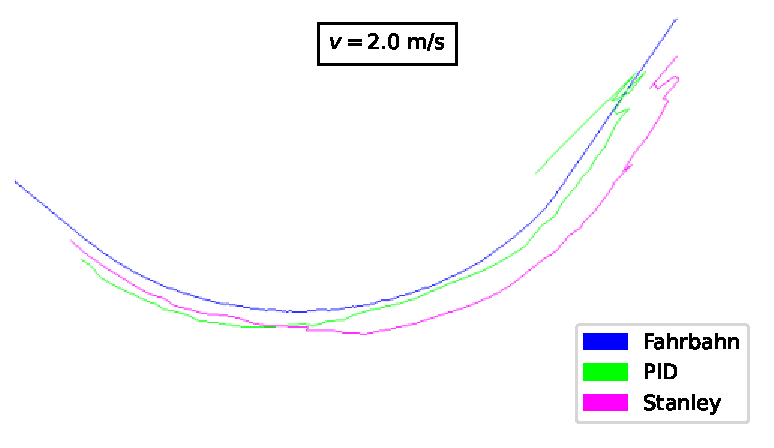
\includegraphics[width=0.9\linewidth]{done2.0}}
        \caption{$v = 2.0 \frac{\mathrm{m}}{\mathrm{s}}$.}
        \label{ab:2.0}
    \end{subfigure}
    \caption{Das Modellfahrzeug mit dem Stanley-Regler hat eine kleine Abweichung am Anfang der Kurve (rechts). Dabei handelt
    es sich um den in Kapitel 4 beschriebenen Drift. Am Ende der Kurve ist es aber auf der Fahrspur.}
\end{figure}

\subsection{Reglerausgang}

Die Ergebnisse des Experiments sind in Tab. \ref{reglerausgabe} aufgef"uhrt.
Die durchschnittliche Reglerausgabe beider Regler ist ähnlich, unabhängig von
der Geschwindigkeit, außer für den PID-Regler bei einer Geschwindigkeit von 1,5
m/s. Mit zunehmender Vorwärtsgeschwindigkeit des Fahrzeugs steigt der
durchschnittliche Reglerausgang f"ur beide Regler an. Der Unterschied zwischen den
beiden Reglern liegt jedoch im zeitlichen Verlauf der beiden Signale. Bei
Vorwärtsgeschwindigkeiten zwischen 1,0 und 1,5 $\frac{\mathrm{m}}{\mathrm{s}}$
ist der Signalverlauf der beiden Regler ähnlich, wie in Abb. \ref{reg:1.0} und
\ref{reg:1.5} zu sehen sind. Bei 1,75 und 2,0 $\frac{\mathrm{m}}{\mathrm{s}}$
verschlechtert sich jedoch der periodische Verlauf des PID-Reglers, während die
Periodizität des Stanley-Reglers zunimmt.

    \begin{table}[h]
\begin{center}
        \begin{tabular}{|c|c|c|}
            \hline
            Geschwindigkeit (m/s) & PID (\textdegree) & Stanley (\textdegree)\\
            \hline
            \hline
            1,0 & 5,33 & 4,79 \\ 
            \hline
            1,25 & 11,97 & 11,82 \\
            \hline
            1,5 & 9,61 & 13,19 \\
            \hline
            1,75 & 12,35 & 13,30 \\
            \hline
            2,0 & 13,84 & 13,51 \\
            \hline
        \end{tabular}
        \caption{Zeitliche Mittelwerte der Reglerausg"ange bei den verschiedenen
        Vorw"artsgeschwindigkeiten.}
        \label{reglerausgabe}
\end{center}
    \end{table}
Bei 1,75 $\frac{\mathrm{m}}{\mathrm{s}}$ kann der PID-Regler das Fahrzeug immer
noch auf die Fahrspur lenken. Wie in Abb. \ref{reg:1.75} gezeigt, führen
Ausreißer allerdings zu starken Schwingungen im Reglerausgang. Wenn der
PID-Regler die Fahrspur nicht richtig erkennt, hat er Schwierigkeiten, das
Fahrzeug auf die Fahrspur zurückzubringen. Stattdessen kann es passieren, dass
das Fahrzeug gegen die Wand fährt, wie am rechten Ende des Diagramms zu sehen
ist. Im Vergleich dazu hat der Stanley-Regler keine Probleme, dem Weg mit der
gleichen Geschwindigkeit zu folgen.

Bei 2,0 $\frac{\mathrm{m}}{\mathrm{s}}$ ist der PID-Regler nicht in der Lage,
eine Kollision mit der Wand zu vermeiden. Wie in Abb. \ref{reg:2.0}
dargestellt, schwankt der Ausgang zwischen -30 und 30 Grad, und es gibt keine
Periodizität. Im Vergleich dazu weist der Stanley-Regler eine stabile
Schwingung zwischen -30 und 0 Grad auf und ist periodisch.

Ausreißer führen nicht zu starken Schwingungen, wenn das Fahrzeug mit dem
Stanley-Regler gesteuert wird. Es wurde beobachtet, dass sich das Fahrzeug viel
schneller als der PID-Regler auf der Bahn neu orientiert.

\begin{figure}[h]
    \centering
    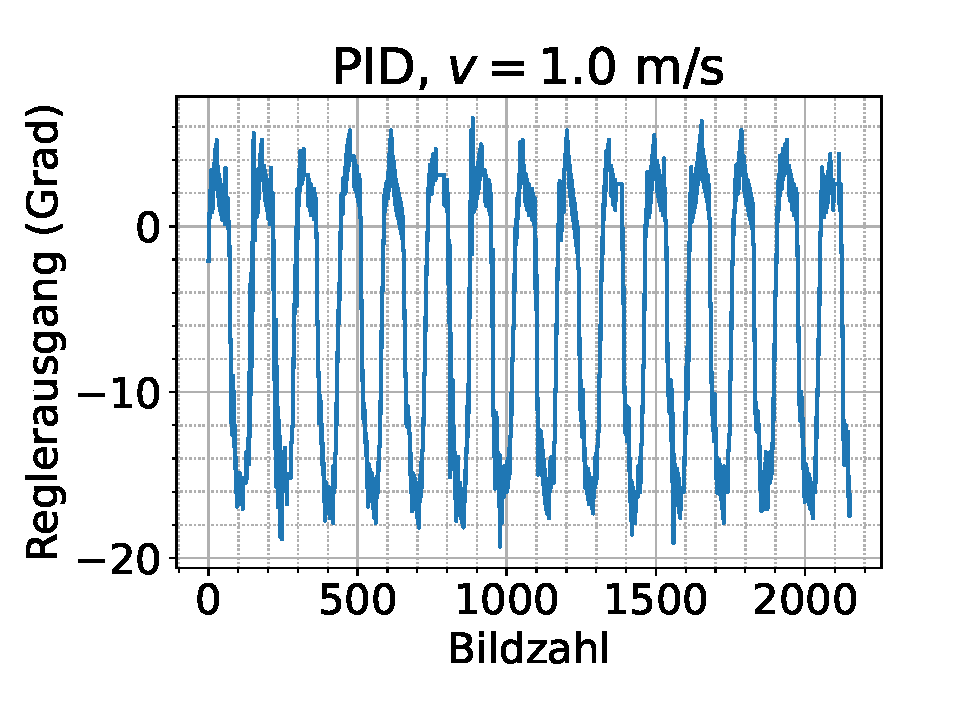
\includegraphics[scale=0.47]{pid1.0}
    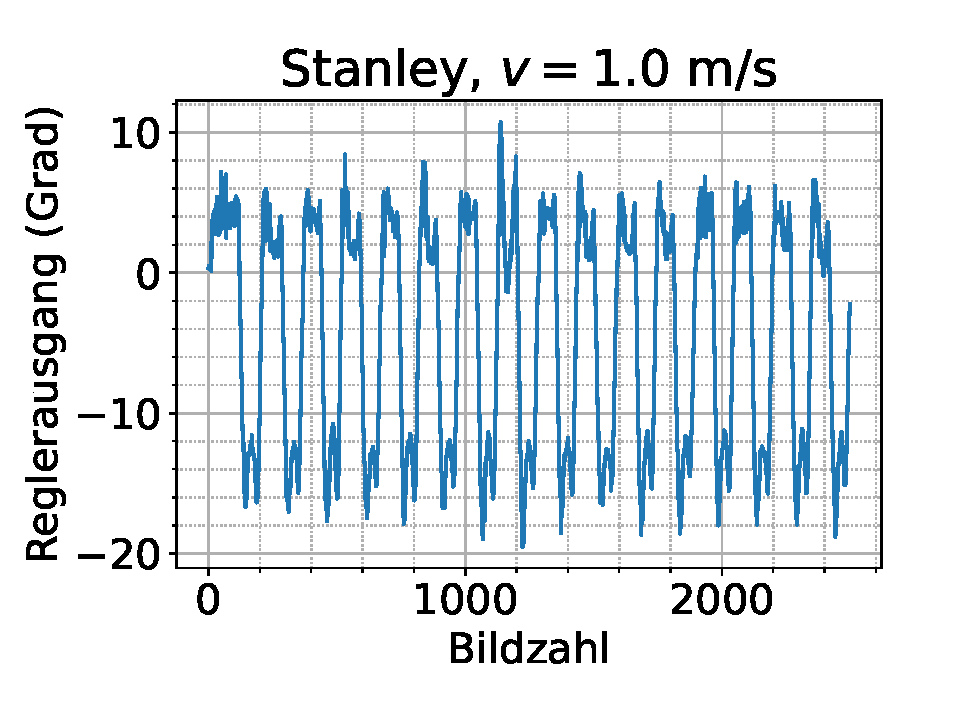
\includegraphics[scale=0.47]{Stan1.0}
    \caption{Ausgang der Regler mit $v = 1.0$ $\frac{\mathrm{m}}{\mathrm{s}}$.}
    \label{reg:1.0}
\end{figure}

\begin{figure}[h]
    \centering
    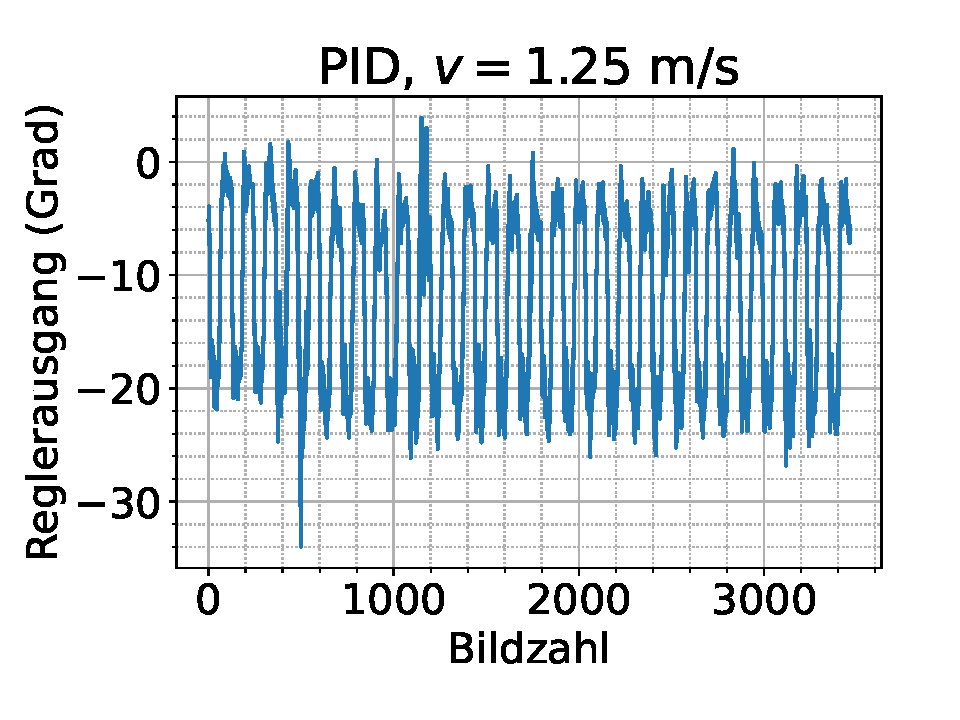
\includegraphics[scale=0.47]{pid1.25}
    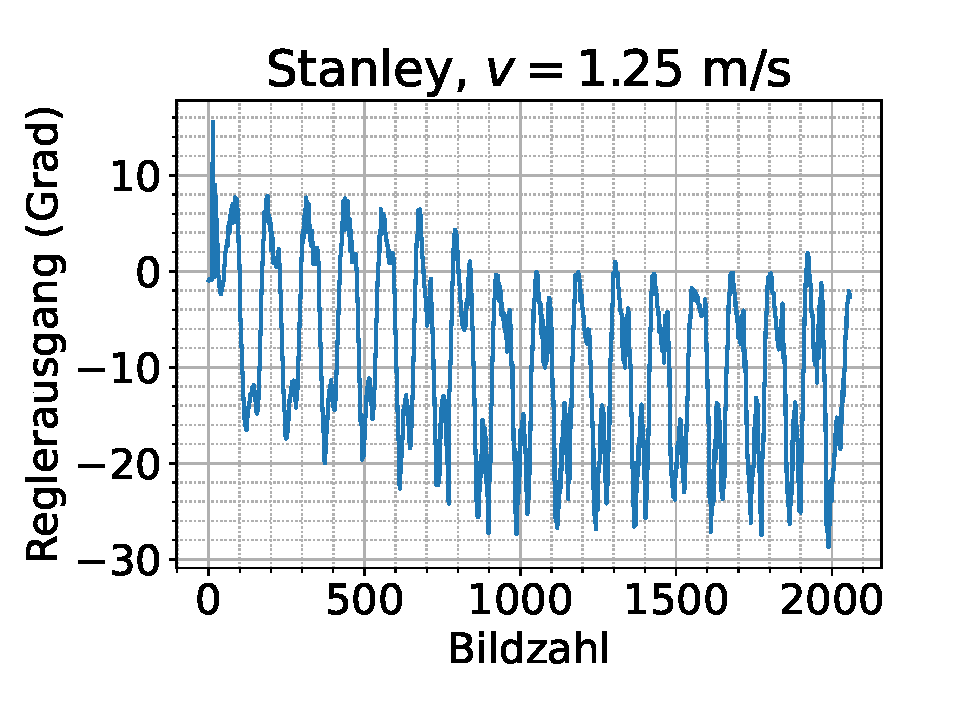
\includegraphics[scale=0.47]{Stan1.25}
    \caption{Ausgang der Regler mit $v = 1.25$ $\frac{\mathrm{m}}{\mathrm{s}}$.}
    \label{reg:1.25}
\end{figure}

\begin{figure}[h]
    \centering
    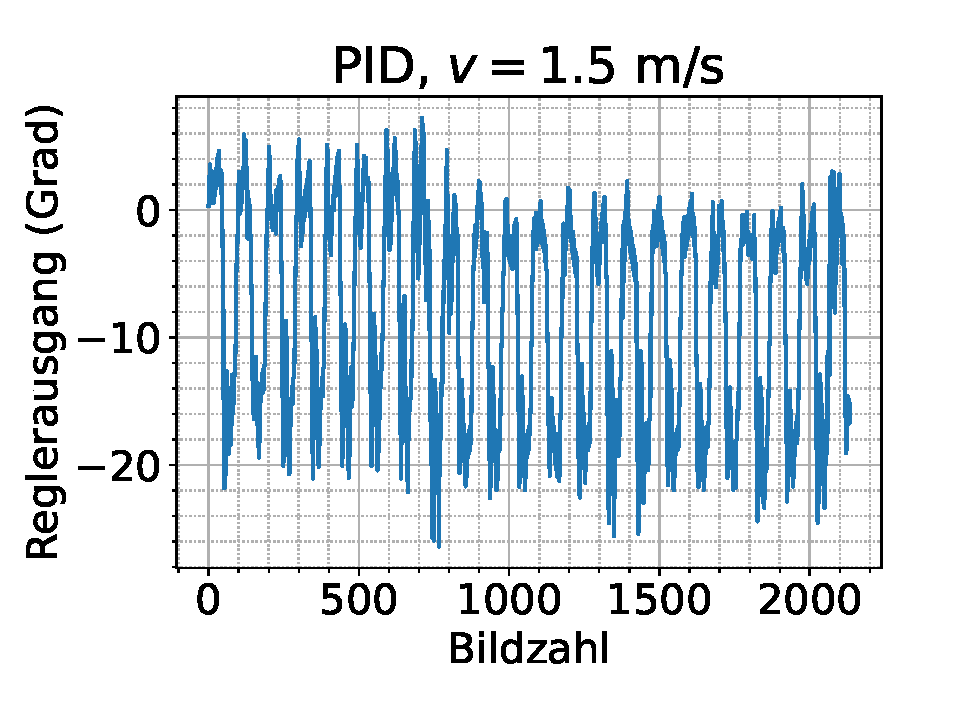
\includegraphics[scale=0.47]{pid1.5}
    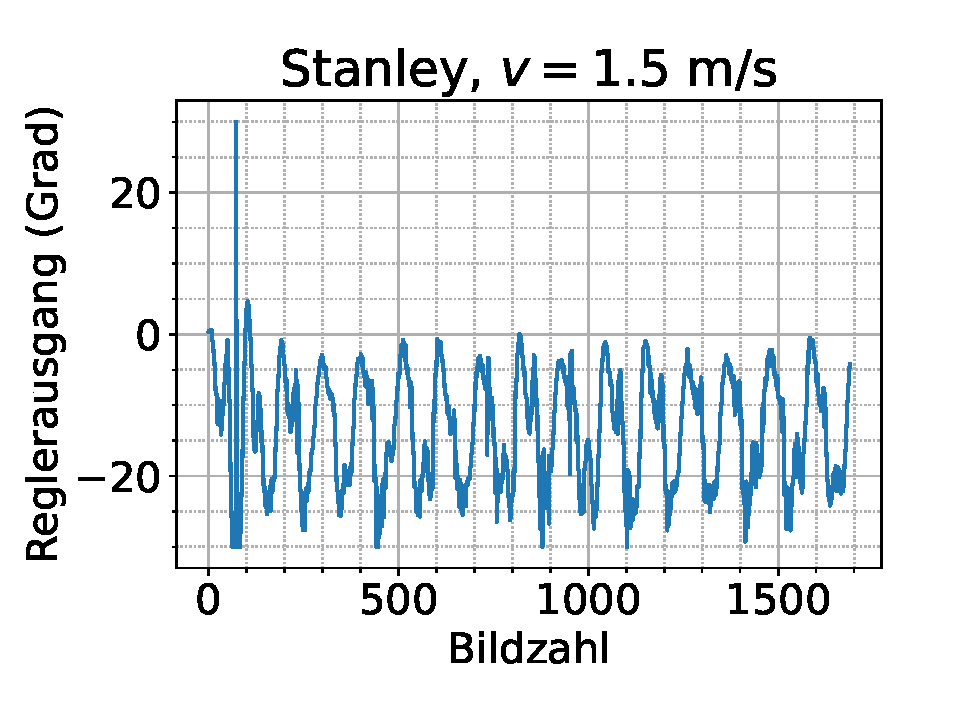
\includegraphics[scale=0.47]{Stan1.5}
    \caption{Ausgang der Regler mit $v = 1.5$ $\frac{\mathrm{m}}{\mathrm{s}}$.}
    \label{reg:1.5}
\end{figure}

\begin{figure}[h]
    \centering
    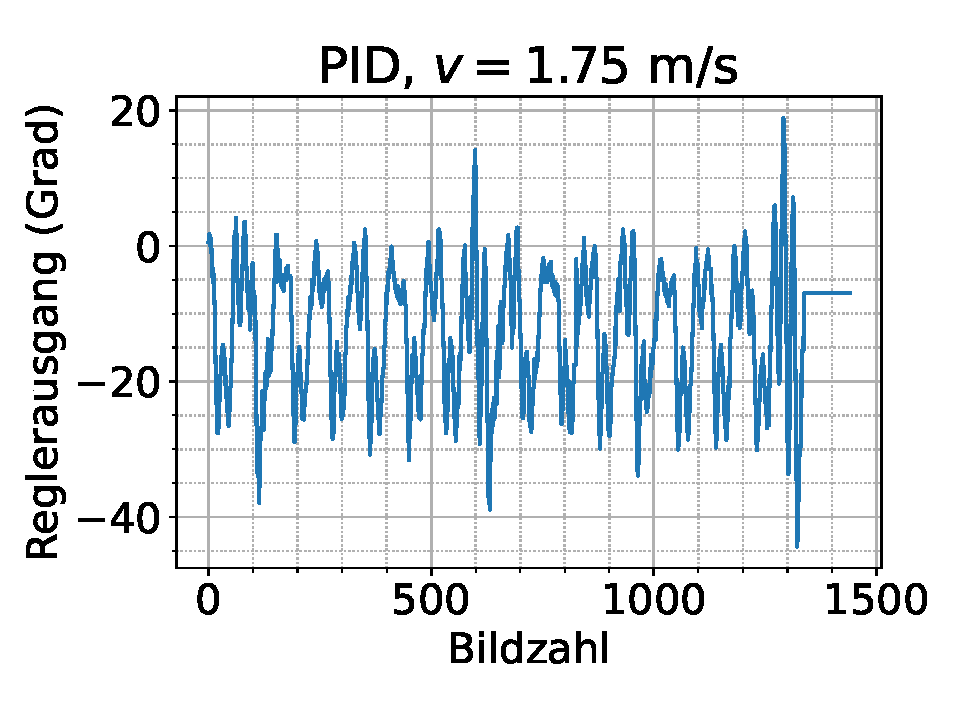
\includegraphics[scale=0.47]{pid1.75}
    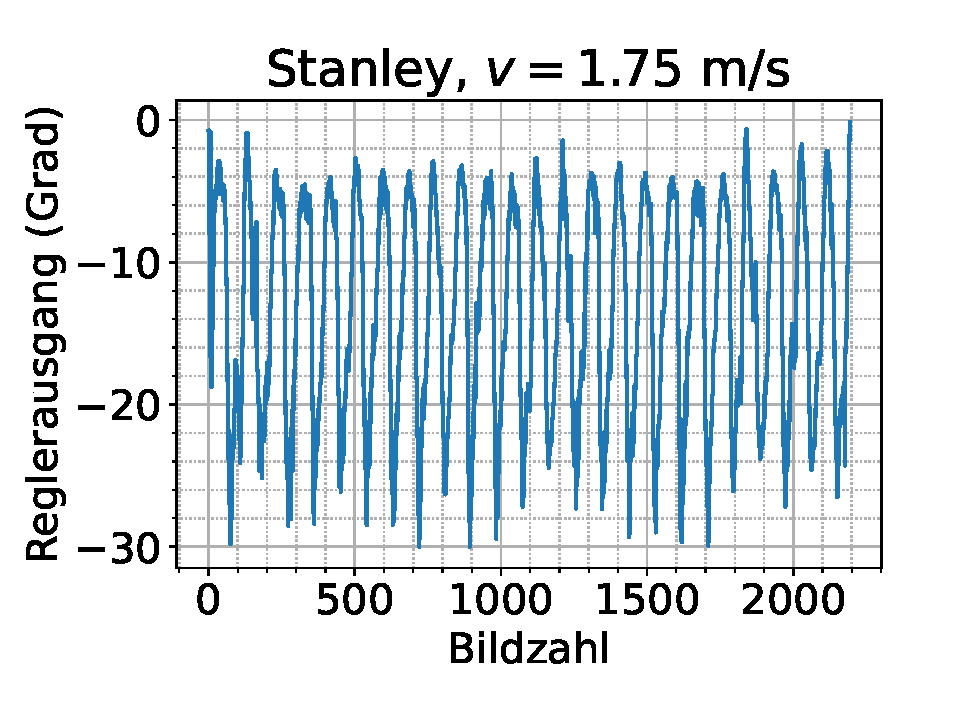
\includegraphics[scale=0.47]{Stan1.75}
    \caption{Ausgang der Regler mit $v = 1.75$ $\frac{\mathrm{m}}{\mathrm{s}}$.}
    \label{reg:1.75}
\end{figure}

\begin{figure}[h]
    \centering
    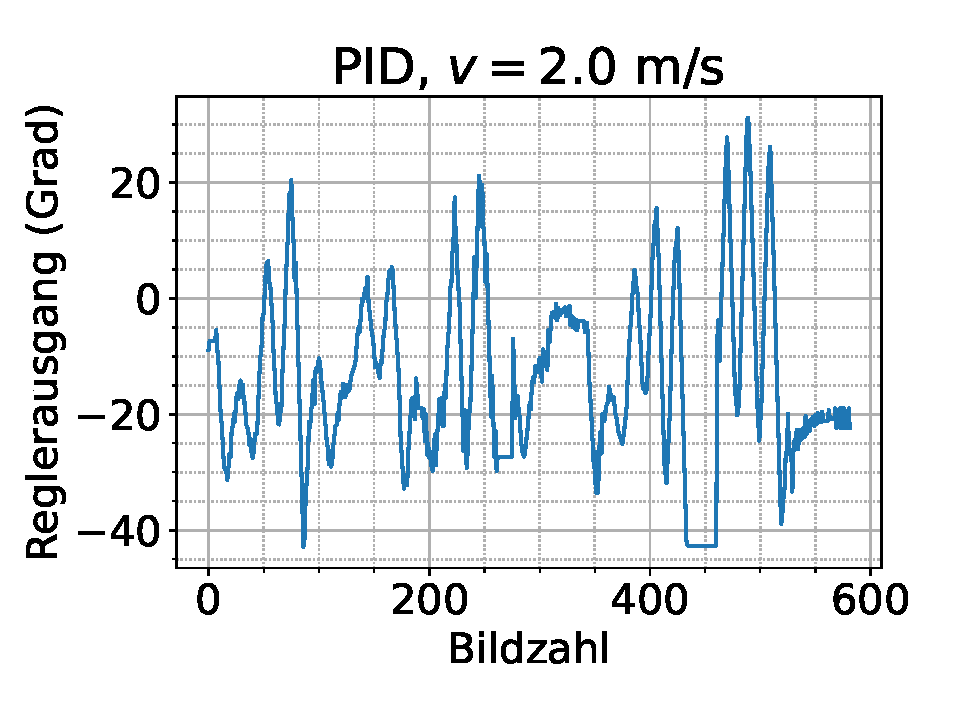
\includegraphics[scale=0.47]{pid2.0}
    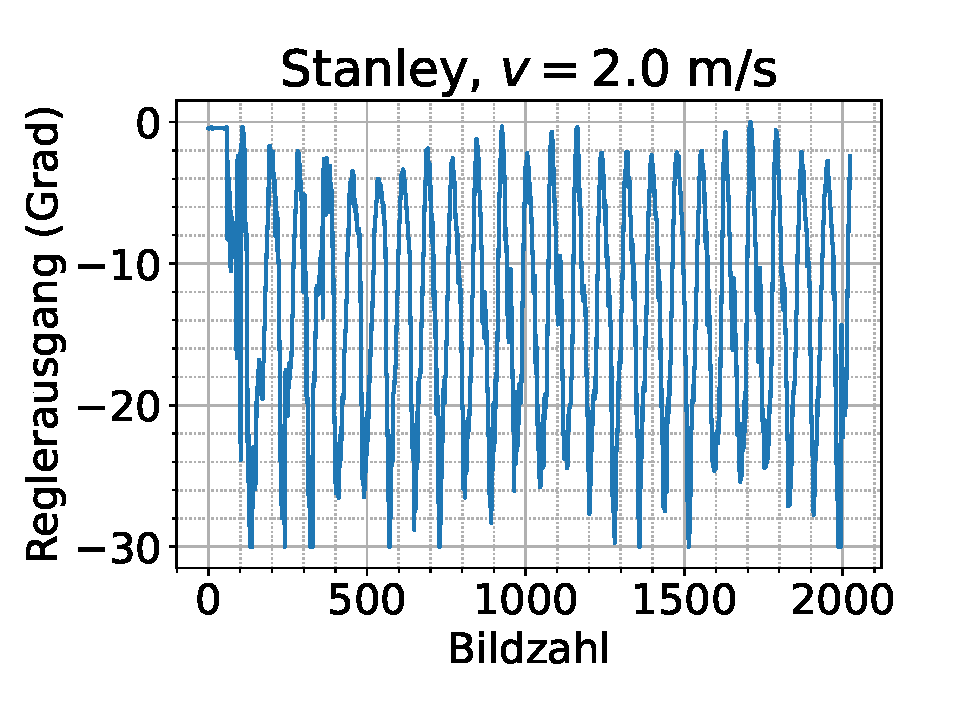
\includegraphics[scale=0.47]{Stan2.0}
    \caption{Ausgang der Regler mit $v = 2.0$ $\frac{\mathrm{m}}{\mathrm{s}}$.
    Das PID-Regler-Signal hat keine Periodizit"at und schwankt von -40 zu 30
    Grad. Er ist bei dieser Geschwindigkeit nicht mehr nutzbar.}
    \label{reg:2.0}
\end{figure}




\chapter{Fazit}

Das Bahnfolgeverhalten beider Regler wurde bewertet. Während der PID-Regler
unter diesem Aspekt besser abschneidet, ist dies nicht das wichtigste Kriterium
bei der Auswahl des Regelungsalgorithmus. Größere Bedeutung ist der Robustheit
zuzumessen. In diesem Kontext hat sich der Stanley-Regler als überlegen
erwiesen. Deshalb ist der Stanley-Regler geeigneter für die Anwendung des
autonomen Fahrens, da er in der Lage ist, höhere Geschwindigkeiten ohne
Überwachung zu bewältigen. Unter Berücksichtigung aller Aspekte der
Problemstellung ist der Stanley-Regler daher die bessere Wahl für diese
Anwendung.




\subsection{K"unftige Arbeit}

Am Ende dieser Arbeit wurde festgestellt, dass das Fahrzeug vor jeder Kurve
immer noch von der Fahrbahn abdriftet. Um dieses Problem zu lösen, wird
vorgeschlagen, den Stanley-Regler in Anlehnung an \cite{iglied} durch
Hinzufügen eines Integrators zu verändern, um diese Abweichung zu kompensieren.
Der adaptierte Stanley-Regler wird durch die folgende Gleichung beschrieben:

\begin{equation}
    u = \theta - \theta_d + \arctan\left(\frac{ke_{V}}{v}\right) + k_{i} \int_{0}^{t} e_{V}d\tau,
    \label{eq:Stanley-Regler-adjusted}
\end{equation}

In der linearen Regelungstheorie wird ein Integrator verwendet, um bleibende
Regelabweichungen aus einer Anwendung zu entfernen. Da es sich bei der
Kleinsignalversion des Stanley-Reglers um einen PD-Regler handelt, ist zu
vermuten, dass das Hinzufügen eines Integrators den beobachteten Drift
korrigieren wird. Wie in der Abb. \ref{quer} zu sehen ist, ist der Drift im Eingang
des Reglers sichtbar. Durch die Integration der Querabweichung soll der Drift
mit der Zeit kompensiert werden und das Fahrzeug auf der Fahrspur bleiben.
Weitere Untersuchungen sind erforderlich, um diese Hypothese zu testen und die
Wirksamkeit der vorgeschlagenen Anpassung zu überprüfen.

\begin{figure}[h]
    \centering
    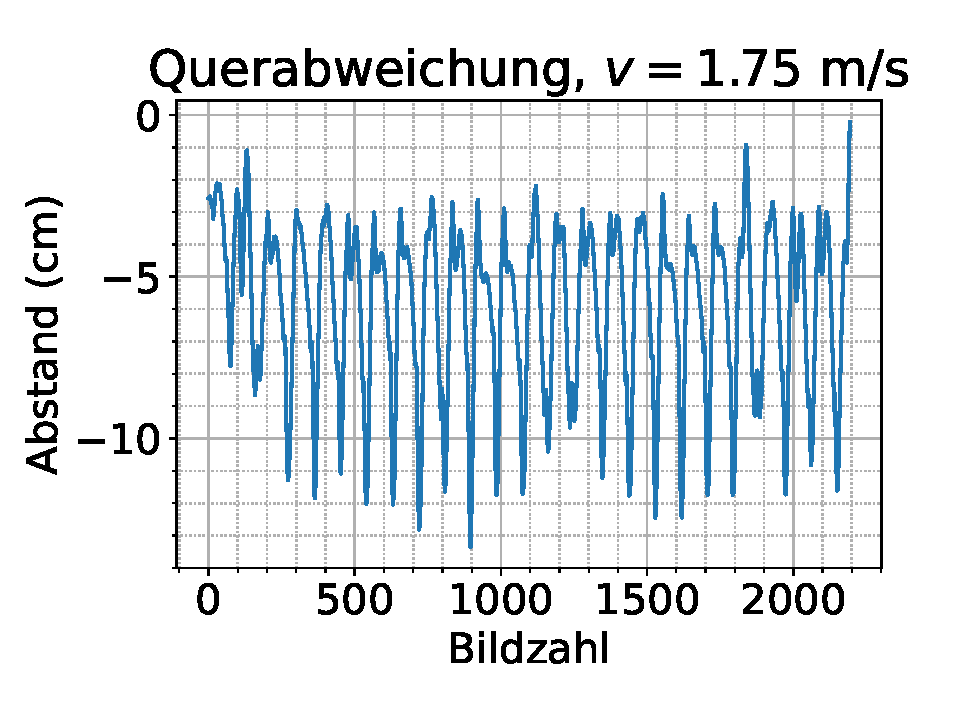
\includegraphics[scale=0.47]{querabweichung}
    \caption{Das gemessene Querabweichungsignal mit $v = 1.75$ $\frac{\mathrm{m}}{\mathrm{s}}$. Der Mittelwert
    des Signals liegt bei -5.89 cm. Deswegen gibt es ein bleibende Abweichung, die 
    mit dem urspr"unglichen Stanley-Regler nicht kompensiert wird.}
    \label{quer}
\end{figure}

\printbibliography

\end{document}
